
This search \cite{Khachatryan:2016kdk} looks for an excess of events
with four or more jets,
no identified and isolated electron, muon,
or isolated charged track,
large $\Ht$, and large $\mht$.
The principal standard model backgrounds are
 events with top quarks,
W bosons and jets,
Z bosons and jets,
and QCD multi-jet production,
and are evaluated using control samples in the data as well 
as information based on simulated events.

The search targets simplified model scenarios corresponding to  
gluino pair production.
In the various models, the gluino decays 100\% of the time into: 
 an LSP and  a light flavor q$\bar{\text{q}}$ pair (T1qqqq model), 
 an LSP and a t$\bar{\text{t}}$ pair  (T1tttt model), 
 an LSP and a b$\bar{\text{b}}$ pair (T1bbbb model).
Also considered is a model in which the gluino decays into
a q$\bar{\text{q}}$ pair and
a next-to-lightest EWkino, $\tilde{\chi}^{0}_{2}$ or $\chi^{\pm}_{1}$ (T5VV model), where 
the masses of the intermediate $\tilde{\chi}^{0}_{2}$ and $\tilde{\chi}^{\pm}_{1}$  states
are taken to be the mean of $m_{\tilde{\chi}^{0}_{1}}$ and $m_{\tilde{\text{g}}}$.
These four models are shown in 
Fig. \ref{fig:Ra2bSMS}.
\begin{figure}[tb!]
\centering
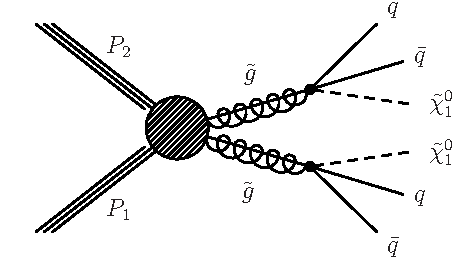
\includegraphics[width=0.45\textwidth]{figures/SusySearches/Ra2b2015/T1qqqq.pdf}
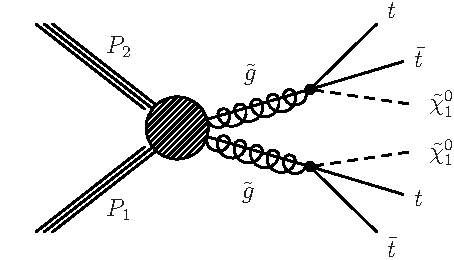
\includegraphics[width=0.45\textwidth]{figures/SusySearches/Ra2b2015/T1tttt.pdf}\\
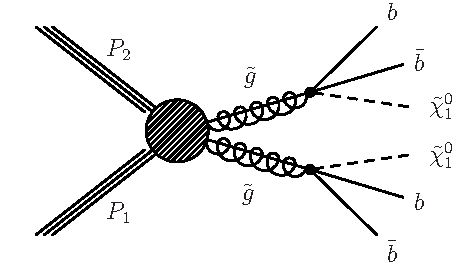
\includegraphics[width=0.45\textwidth]{figures/SusySearches/Ra2b2015/T1bbbb.pdf}
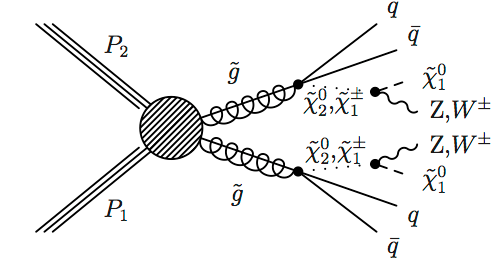
\includegraphics[width=0.45\textwidth]{figures/SusySearches/Ra2b2015/T5vv.pdf}
\caption{
  The simplified models used for the optimization and interpretation of the multi-jet $+$ $\mht$ search. 
  They are T1qqqq (upper left), T1tttt (upper right), T1bbbb (lower left), and T5VV (lower right) scenarios.
}
\label{fig:Ra2bSMS}
\end{figure}

Events are collected using the hadronic trigger
\begin{itemize}
  \item \texttt{HLT\_PFHT350\_PFMET100\_*},
\end{itemize}
where PFHT and PFMET refer to the online $\Ht$ and $\met$ computed using the particle flow (PF) algorithm (Section \ref{sec:reconstruction}), and the numbers 350 and 100 refer to the respective triggering thresholds in units of GeV.

At level 1 of the trigger system, events are triggered if they have a calorimeter-based $\Ht$ of 175 GeV. If the event is accepted, the HLT trigger then requires a calorimeter-based $\Ht>$ 280 GeV and a calorimeter-based $\met>$ 70 GeV. Finally, the HLT trigger applies a lower threshold of 350 GeV on the $\Ht$ in coincidence with a threshold on the $\met$ above 100 GeV computed using all particles reconstructed from information from the tracker and calorimeters.

\begin{figure}[tb!]
  \begin{center}
    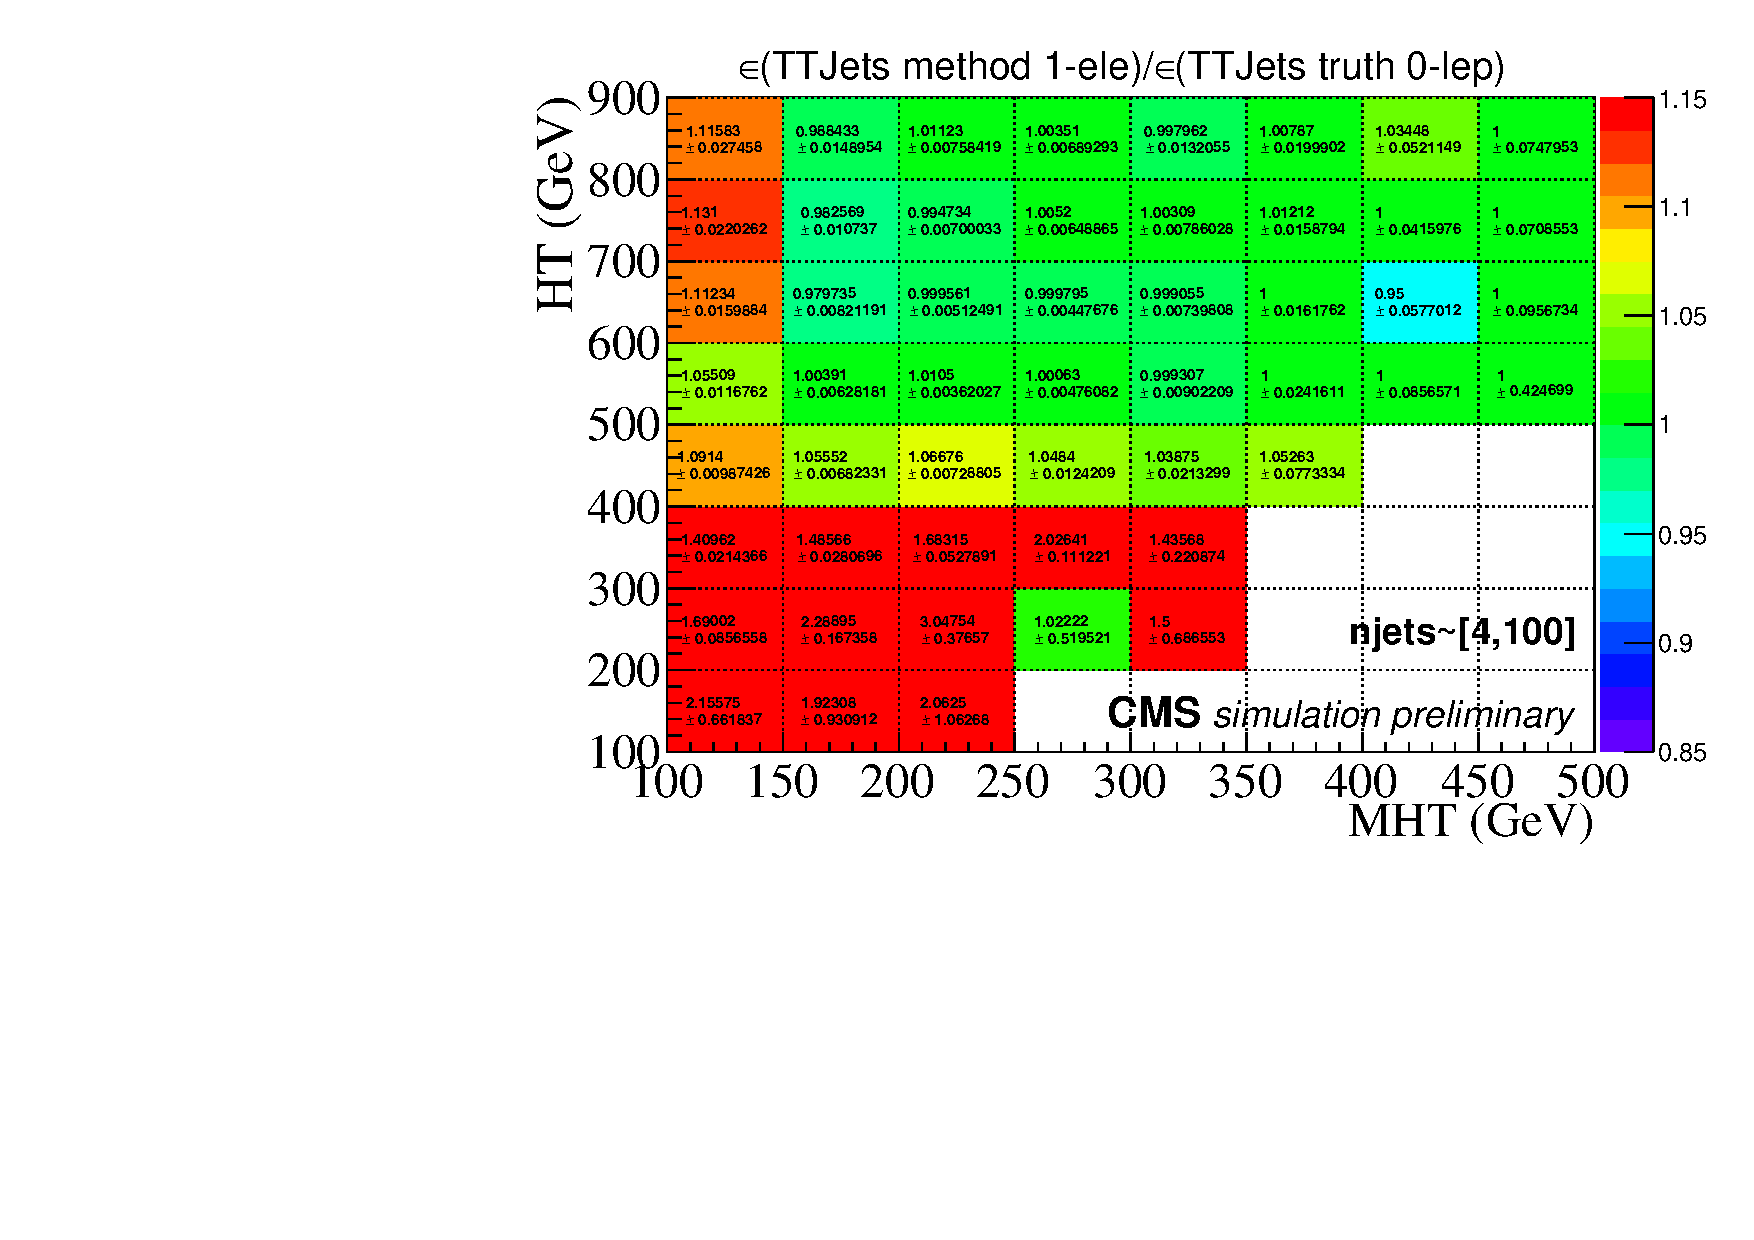
\includegraphics[width=0.95\linewidth]{figures/trigger/EfficiencyRatioMethodTruth.pdf}
    \caption{
      The ratio of the trigger efficiency for events passing the single
      electron reference trigger to the trigger efficiency for all
      events in a simulated t$\bar{\text{t}}$ sample, as a function of the offline $\Ht$
      and $\mht$. The ratio is consistent with 1 within the region of
      the baseline selection of $\Ht>500$ GeV and $\mht>200$ GeV of the CMS hadronic searches.
    }
    \label{fig:2dEffRatio}
  \end{center}
\end{figure}
It is seen that the choice of reference trigger, namely the single electron trigger,
\begin{itemize}
  \item \texttt{HLT\_Ele27\_eta2p1\_WPLoose\_Gsf\_v*}, 
\end{itemize}
allows for an unbiased estimate of the trigger efficiency in the region $\mht>150$ GeV and $\Ht>500$. The region in which the efficiency can be measured without bias includes the baseline selection, which imposes thresholds on the offline $\mht$ and $\Ht$ of 200 and 500 GeV. 

The efficiency, estimated without bias using Equation \ref{eq:trigeff}, is shown as a function of the offline $\Ht$ and $\mht$ in Fig. \ref{fig:trigger-turnon}, where the entire 2015 dataset has been used. 
\begin{figure}[tb!]
  \begin{center}
    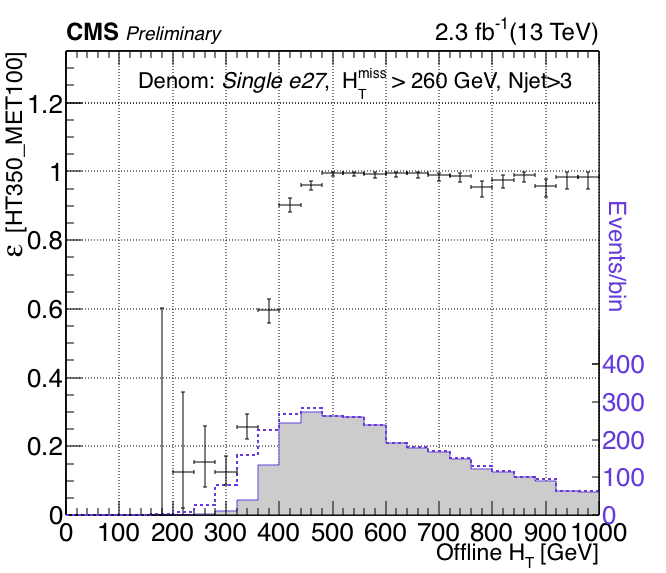
\includegraphics[width=0.49\linewidth]{figures/trigger/EffVsHt2_3InvFb.png}
    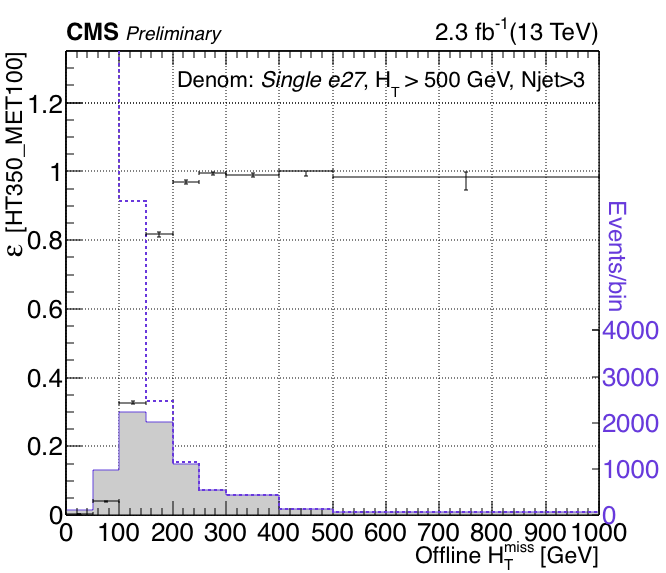
\includegraphics[width=0.49\linewidth]{figures/trigger/EffVsMht2_3InvFb.png}
    \caption{
      The trigger efficiency for \texttt{HLT\_PFHT350\_PFMET100*} 
      as a function of the search variables $\Ht$ and $\mht$. The dashed (solid) blue
      lines show the distributions of the denominator (numerator) samples. These results were used in the CMS PAS on the commissioning of 13 TeV observables for SUSY searches~\cite{CMS-DP-2015-035}.
      }
    \label{fig:trigger-turnon}
  \end{center}
\end{figure}
The statistical uncertainties in the plot correspond to the 68\% CL Clopper-Pearson
interval~\cite{Clopper:Pearson}. Additionally, a systematic uncertainty is assigned to the efficiency
equal to the difference between the efficiency obtained from applying the method described to a
sample of simulated t$\bar{\text{t}}$ events and that derived
from a set of simulated signal events. Such discrepancies may arise due to any number of subtle differences in the content of the events in t$\bar{\text{t}}$ and signal samples. 

The probability for the trigger to fire on an event that passes the baseline selection is greater than 97\%. The baseline event selection can be summarized as follows. Events are accepted if they have
\begin{itemize}
\item no reconstructed, isolated lepton with a $\pt>10$ GeV and $|\eta|<2.4$, where the isolation is as defined in Equation \ref{eq:isolation};
\item no reconstructed, isolated particle track with a $\pt>10$ GeV and $|\eta|<2.4$;
\item $\Ht>500$ GeV;
\item $\mht>200$ GeV;
\item $\njets\geq$ 4, where jets are required to have a $\pt>30$ GeV and $|\eta|<2.4$, and
\item $\Delta\phi(\mht$, jet$_{1,2,3,4})>$ 0.5, 0.5, 0.3, 0.3.
\end{itemize}
After this selection, events are further subdivided into 72 exclusive bins
in a four-dimensional array of $\mht$,
the number of jets,
the number of tagged bottom quark jets,
and $\Ht$. Figure \ref{fig:ra2bArray} shows the boundaries of 6 bins in the $\Ht-\mht$ plane, and 12 bins in the plane of $\njets$$-$$\nbjets$. The 72 bins included in this search are defined by each unique combination of a box in the $\mht$$-$$\Ht$ plane and a box in the $\njets$$-$$\nbjets$ plane. The bin numbering scheme is given in Appendix \ref{app:anatables}.
\begin{figure}[tb!]
\centering
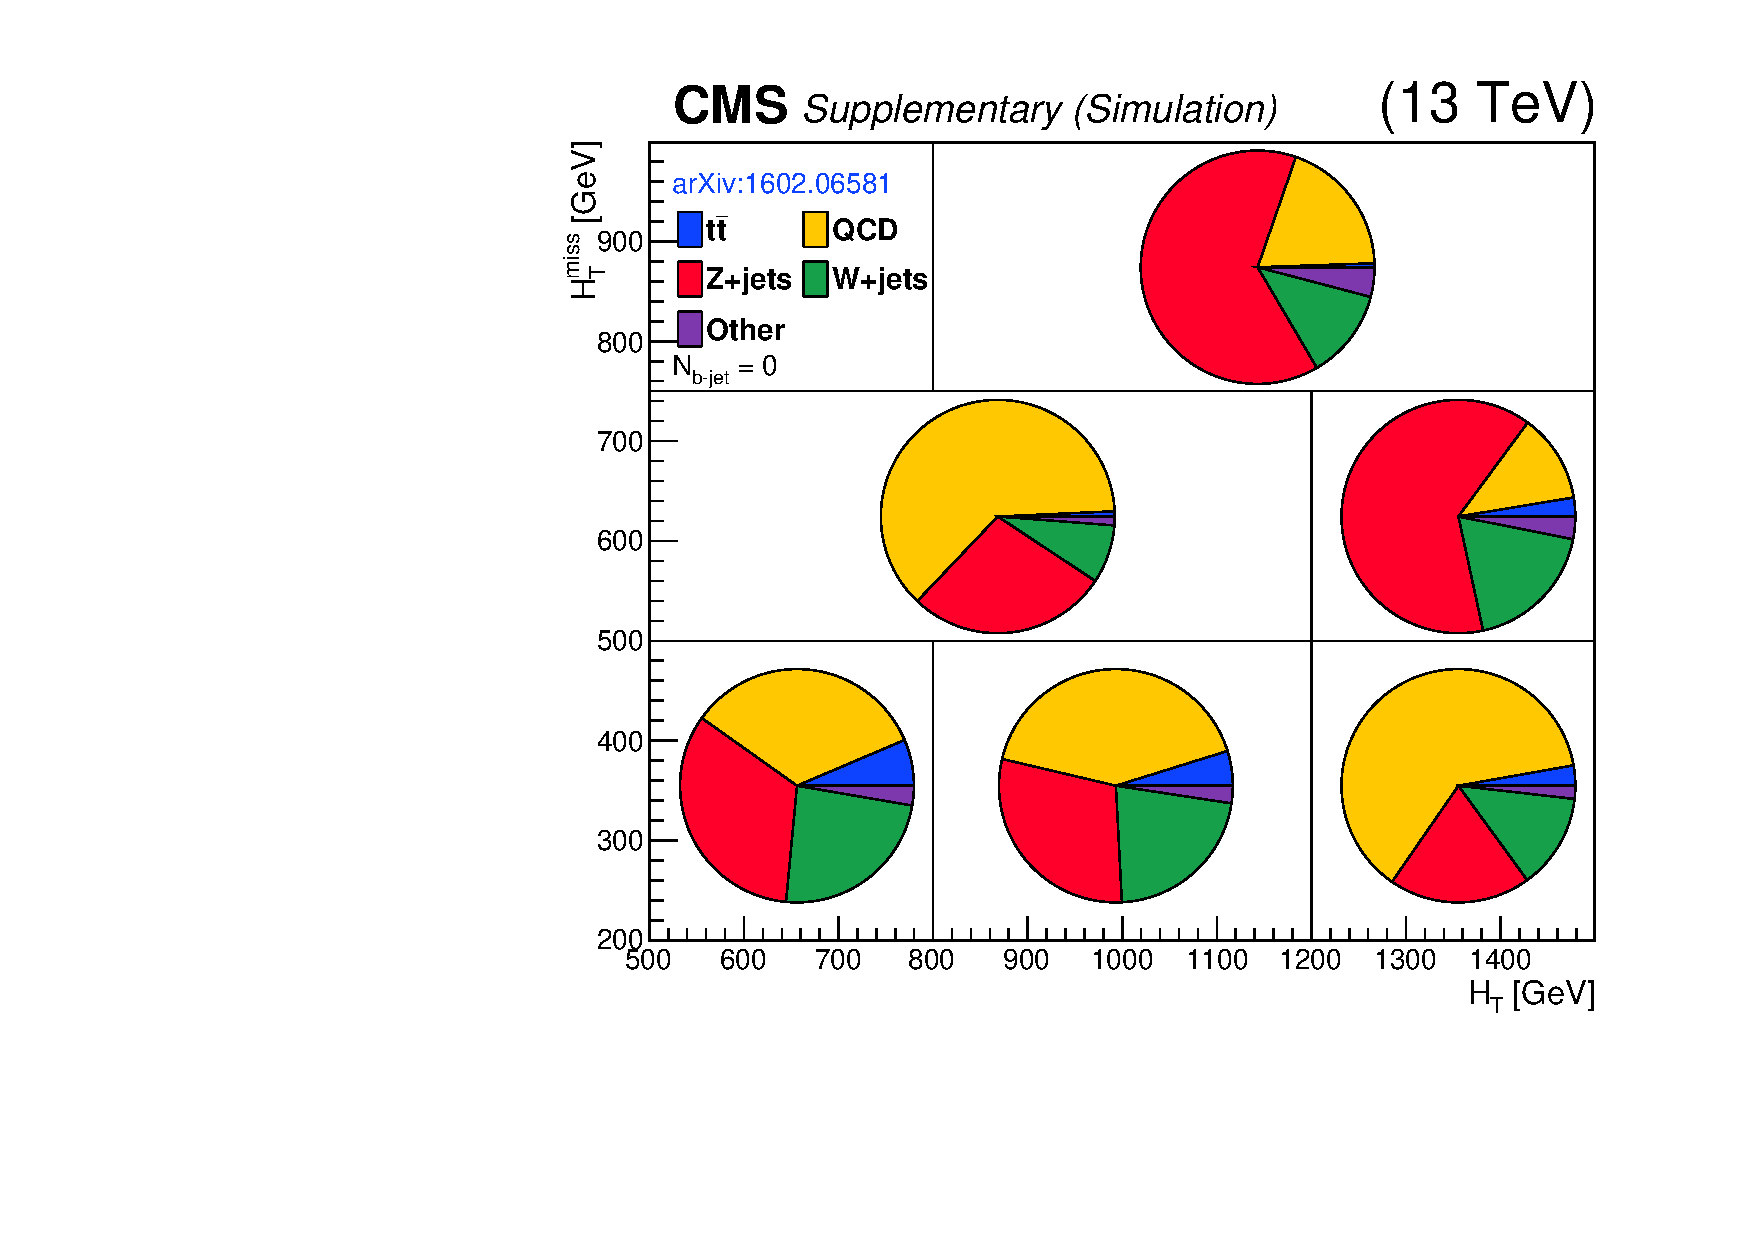
\includegraphics[height=0.442\textwidth]{figures/SusySearches/Ra2b2015/aux/MC_BG_Pie_NB0.pdf}
\hspace{-1cm}
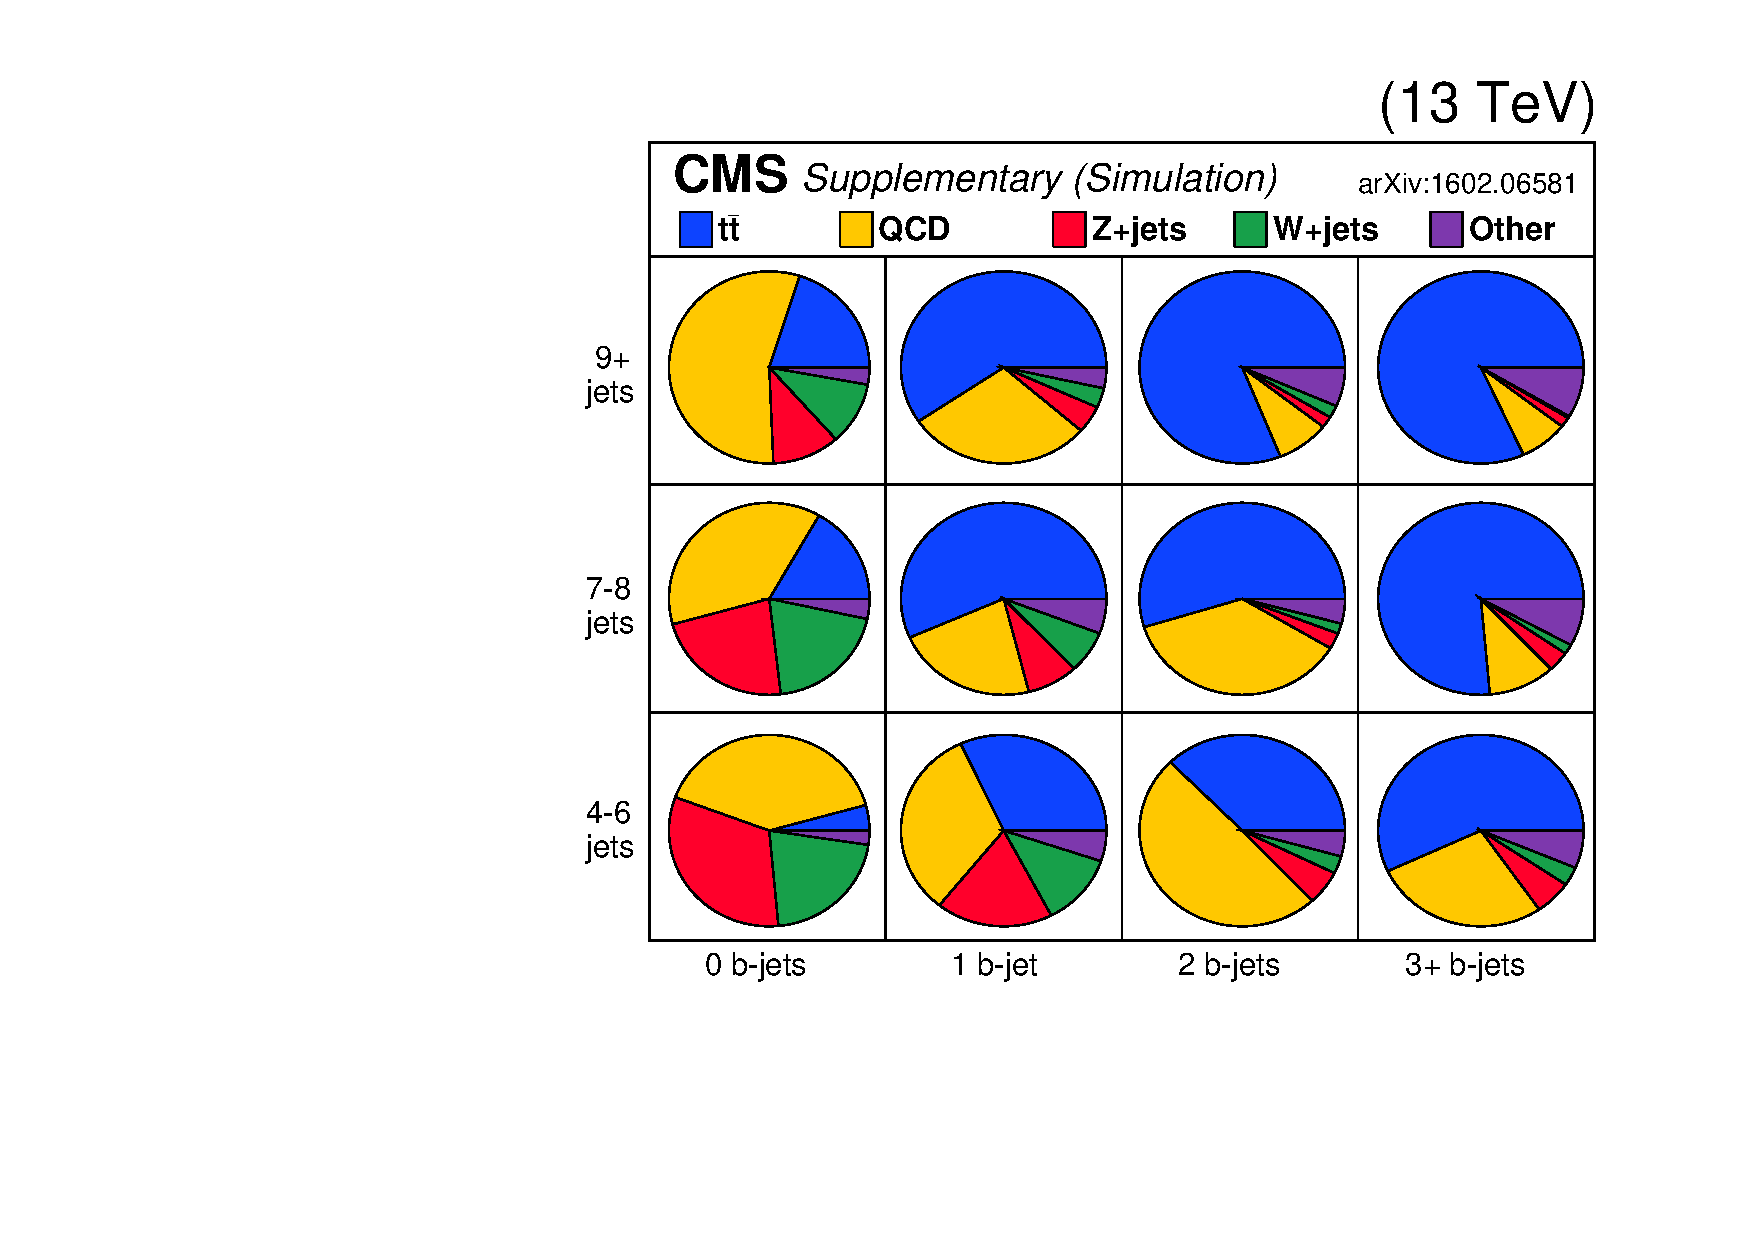
\includegraphics[height=0.445\textwidth]{figures/SusySearches/Ra2b2015/aux/MC_BG_Pie_vs_NJets_NBJets.pdf}
\caption{The signal region boundaries in the planes of $\mht$$-$$\Ht$ (top) and $\njets$$-$$\nbjets$ (bottom) for the multi-jet $+$ $\mht$ 
search. The pie charts represent the relative contributions
 to the~\sm~backgrounds in the region $\njets=$ 4$-$6, $\nbjets=0$ (top), and $\mht=$ 200$-$500 GeV, $\Ht=$ 500$-$750 GeV (bottom).}
\label{fig:ra2bArray}
\end{figure}


\subsubsection{Background estimation}
The relative contribution of each standard model background in selected regions is also shown in Fig. \ref{fig:ra2bArray}. The t$\bar{\text{t}}$, W$+$jets, and Z$+$jets backgrounds are estimated by data-driven methods detailed in  \cite{Khachatryan:2016kdk}, but are not discussed thoroughly here. The QCD background is largest in regions of low $\mht$ and high $\Ht$, and its bin-by-bin estimation is detailed here.

The QCD background is estimated using two independent data-driven methods, one making use of a control region defined analogously to the baseline selection but with the $\Delta\phi$ requirement inverted, and by the rebalance and smear method described in Section \ref{sec:qcd}. The two methods are considered independent because the predictions are derived from nearly disjoint data control samples, and because they use different methodology. 

In the $\Delta\phi$ method, the counts in the inverted $\Delta\phi$ control region are related to the counts in the signal region by factors derived using a combination of input from real and simulated data. The information from the real data comes from events in the least sensitive search bins so as to minimize potential signal contamination. In this method, other standard model backgrounds are subtracted using estimates derived by the data-driven methods employed in the search. The largest sources of uncertainty come from the estimates of the standard model backgrounds that are subtracted. Further details about the inverted $\Delta\phi$ method are given in the literature.

The bin-by-bin prediction based on the rebalance and smear method, along with the systematic uncertainties described in Section \ref{sec:qcd}, are shown in Fig. \ref{fig:2015CompareQCD}, with the predictions and uncertainties based on the inverted $\Delta\phi$ method superimposed. The uncertainties in the rebalance and smear counts are derived based on the methodology described in Section \ref{sec:qcd}. For rebalance and smear, the largest uncertainty in bins with a large count is the uncertainty in the jet energy resolution, ranging from 10$-$30\%. In bins with exceptionally small predicted counts, the statistical uncertainty is dominant, ranging from 20$-$40\%. In bins with three or more b-tagged jets, the non-closure uncertainty is the largest, at 50\%. 
\begin{figure}[tb!]
\centering
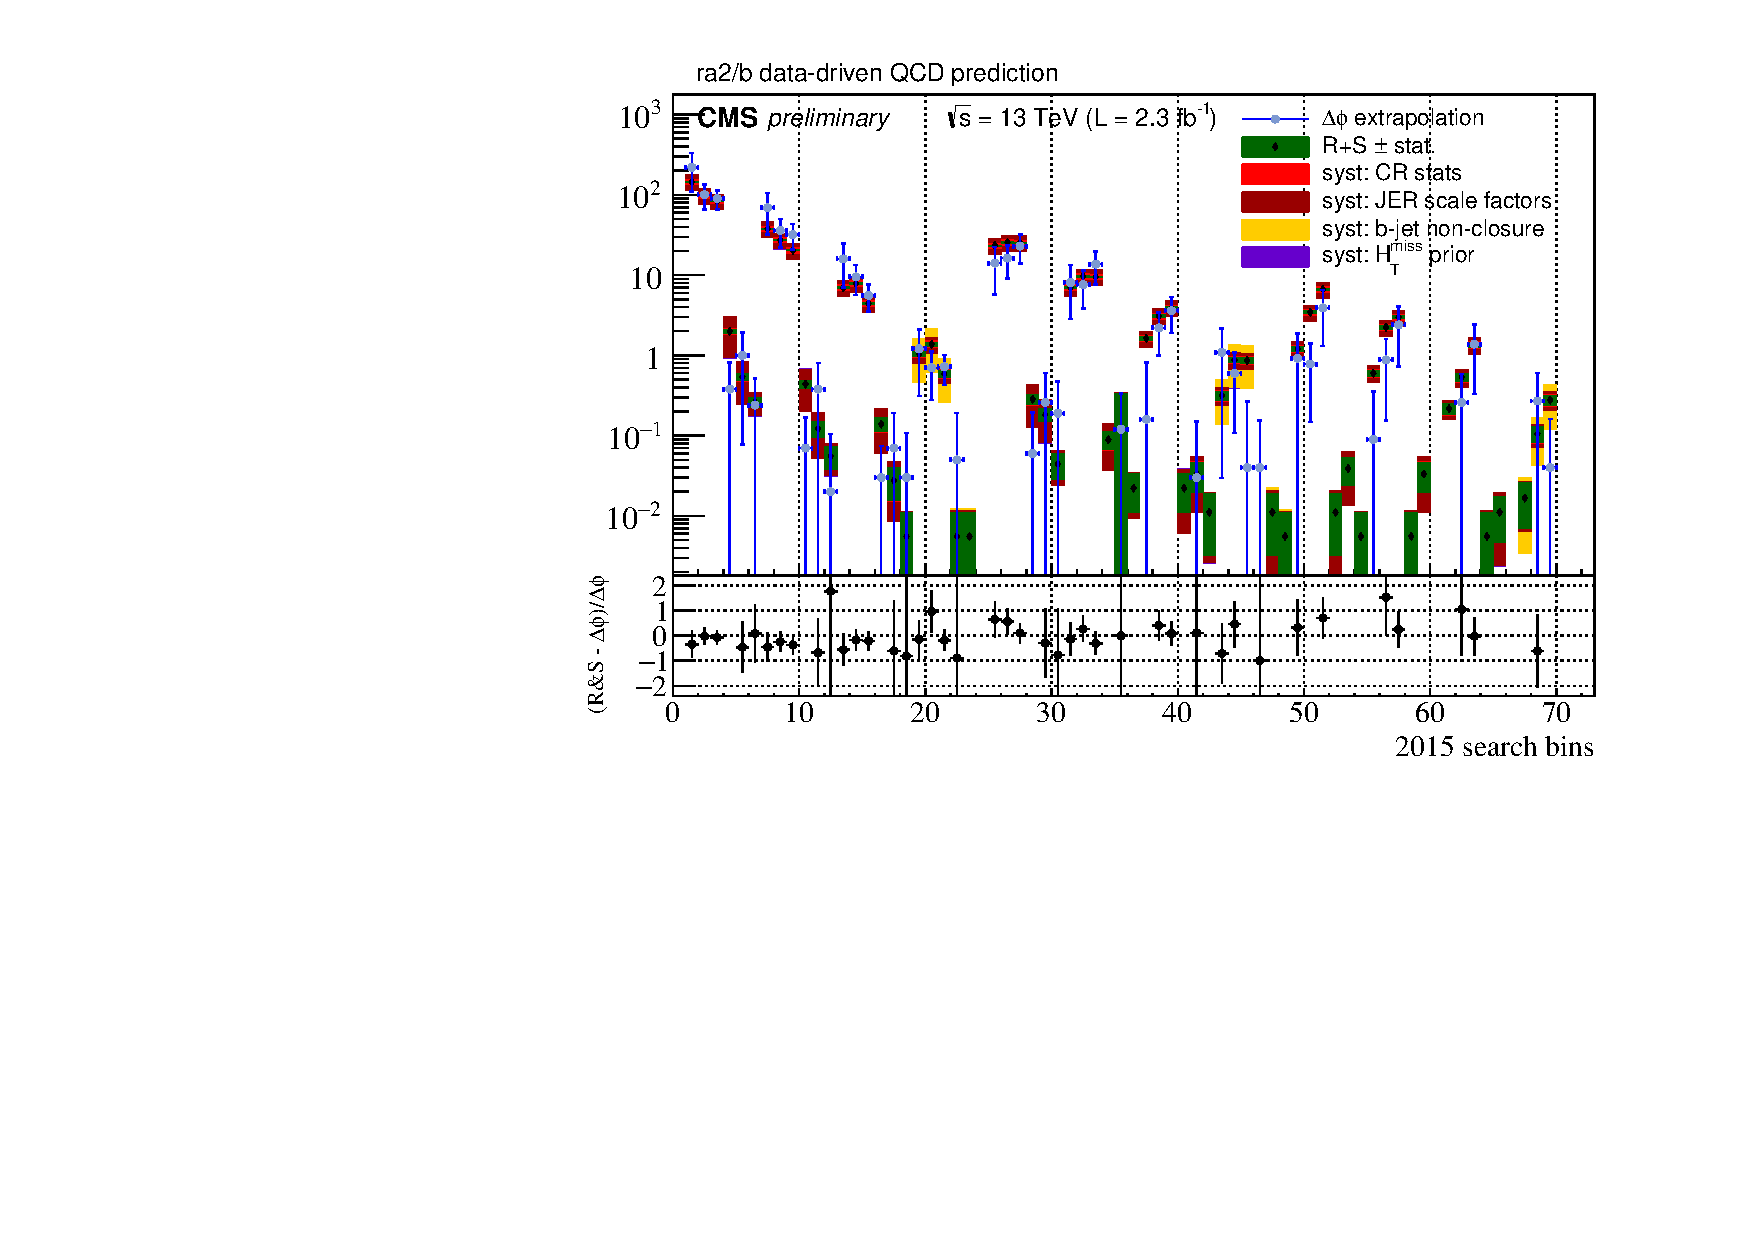
\includegraphics[width=\linewidth]{figures/SusySearches/Ra2b2015/2015CompareQCDErrors.pdf}
\caption{ The QCD prediction based on the inverted $\Delta\phi$ extrapolation method compared with that of the of rebalance and smear method. Each type of uncertainty in the rebalance and smear prediction appears as a color-filled rectangle centered on the predicted value, summed in quadrature with the inner uncertainties. Uncertainties in the inverted $\Delta\phi$ prediction are the statistical systematic uncertainties reported in \cite{Khachatryan:2016kdk}, summed in quadrature.}
\label{fig:2015CompareQCD}
\end{figure}

No evidence of inconsistency is seen between the two predictions. The distribution of the fractional differences in the predictions of the two methods, divided by the uncertainty in the fraction (significance), is shown in Fig. \ref{fig:fractionalUnc} (a). After fitting the significance distribution  with a Gaussian function, as shown in the Figure, the best fit values for the mean and standard deviation indicate consistency between the two predictions.
\begin{figure}[tb!]
\centering
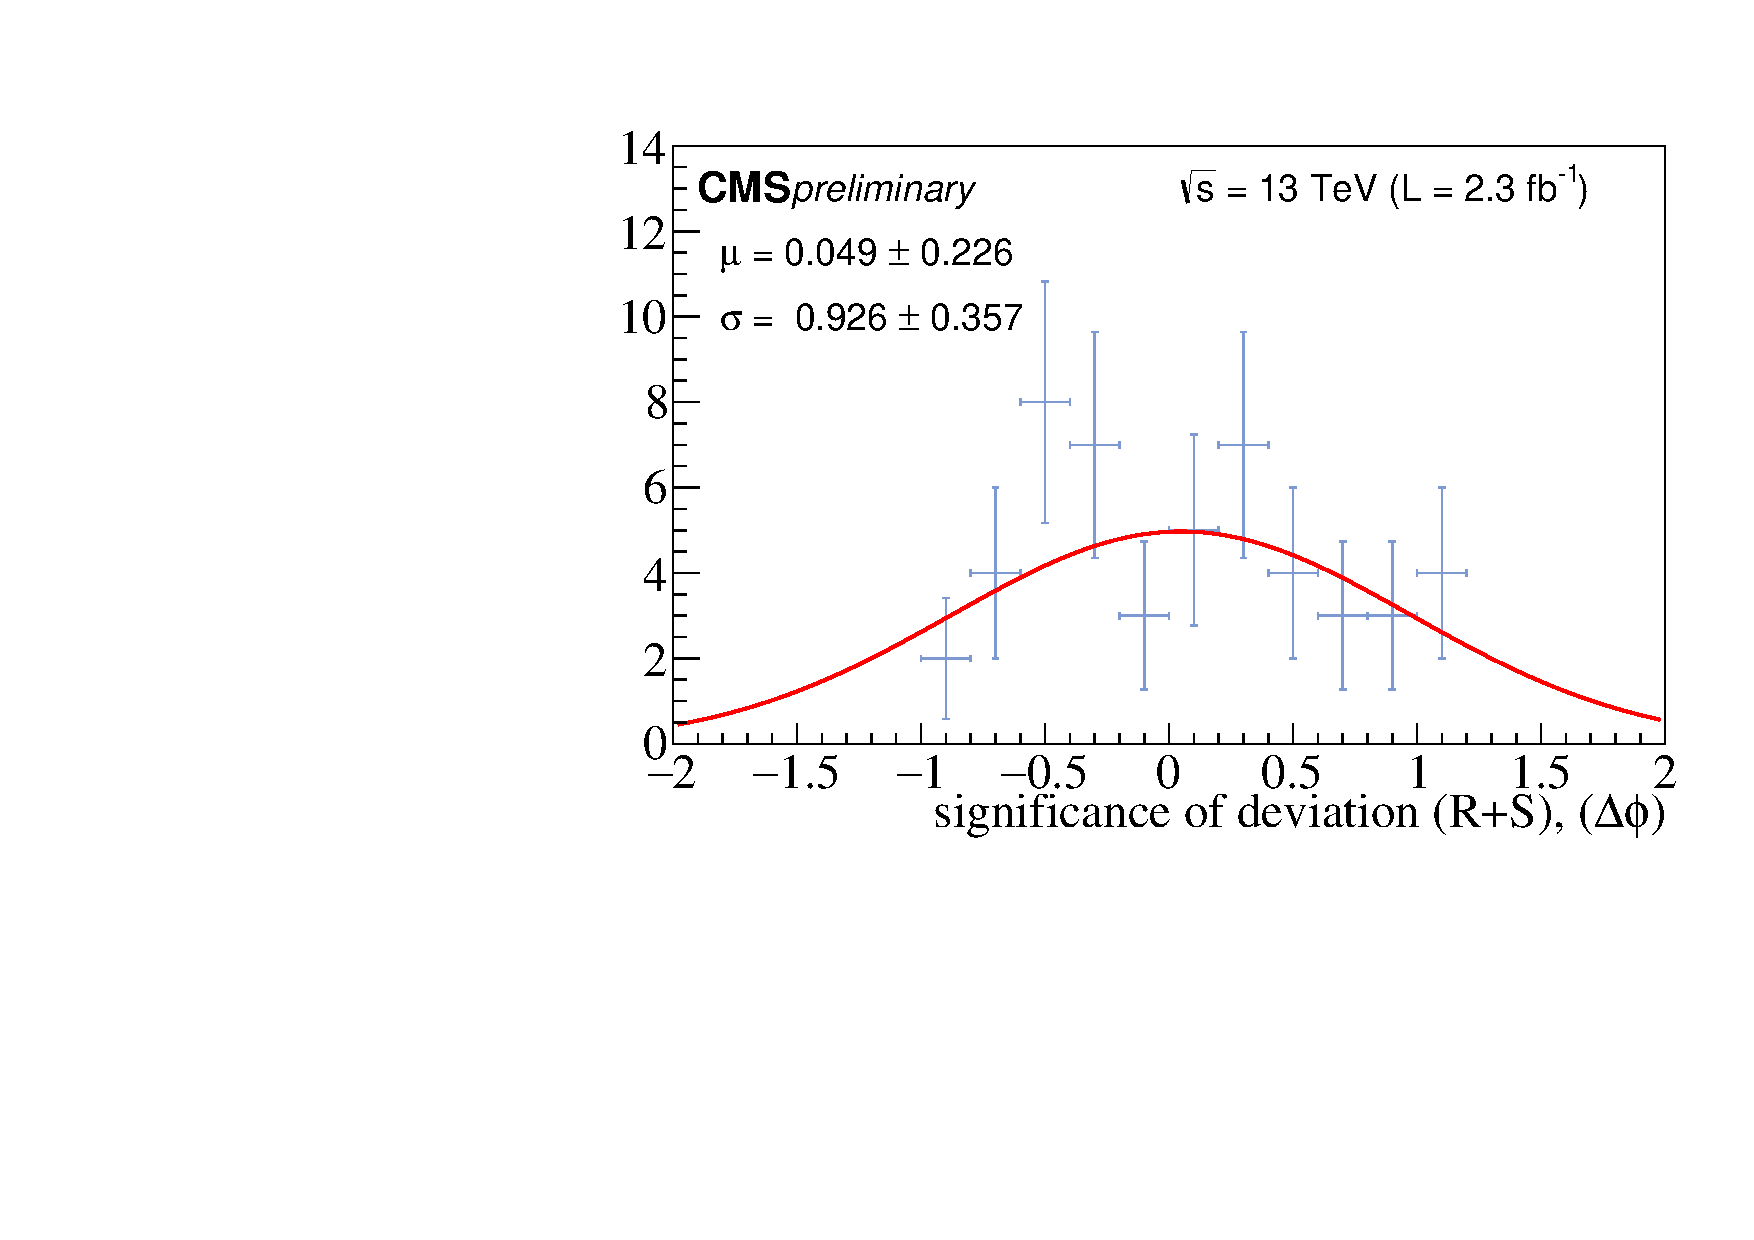
\includegraphics[width=0.49\textwidth]{figures/SusySearches/Ra2b2015/FractionalUncertainty.pdf}
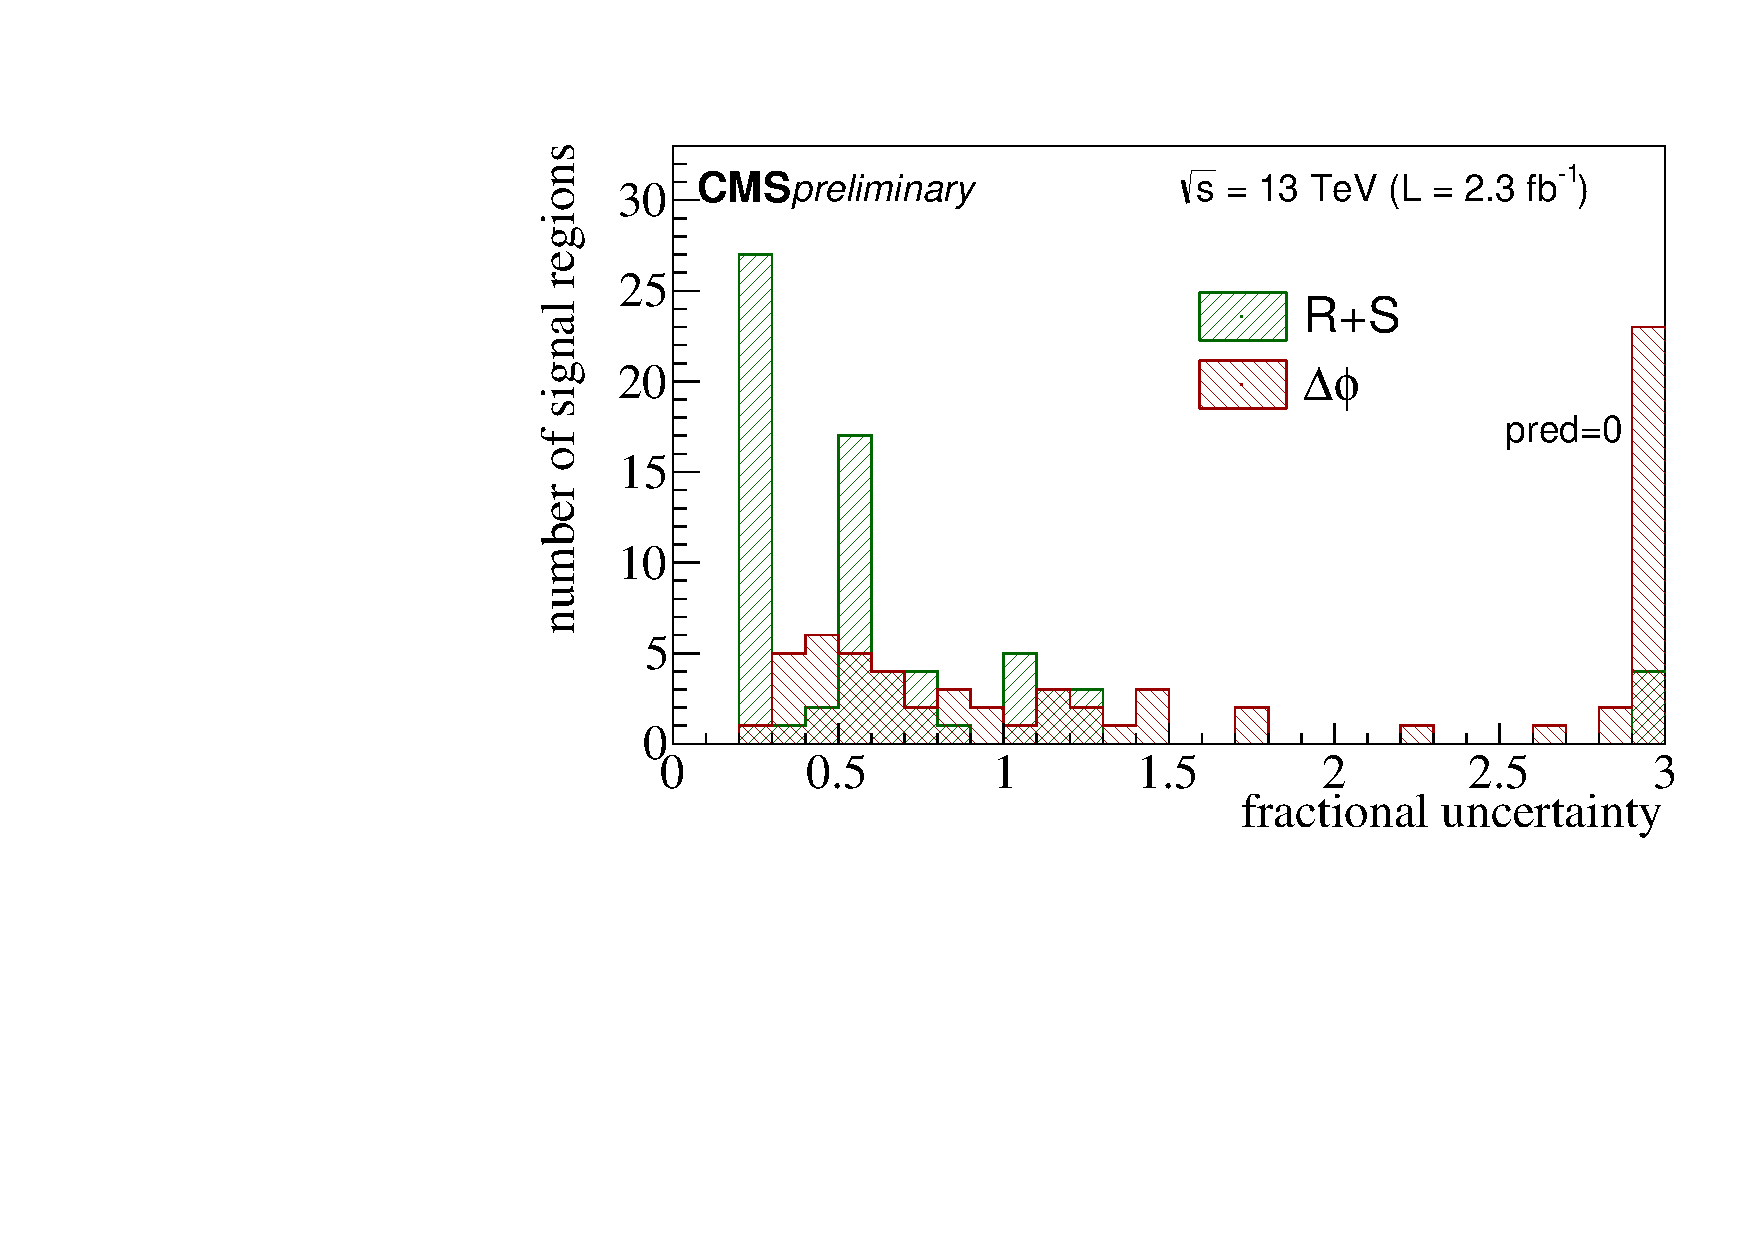
\includegraphics[width=0.49\textwidth]{figures/SusySearches/Ra2b2015/FracUnc.pdf}
\caption{Left: the distribution of the significance of the deviation between the predictions from the inverted $\Delta\phi$ and rebalance and smear methods. Right: the distribution of the fractional uncertainties in the counts predicted by the two methods. The upper overflow bin is populated by bins for which the prediction is identically 0. }
\label{fig:fractionalUnc}
\end{figure}
Fig. \ref{fig:fractionalUnc} (b) shows the distribution of fractional uncertainties in the inverted $\Delta\phi$ and rebalance and smear predictions. It is seen that the inverted $\Delta\phi$ method has a prediction of zero for 22 of the search bins, whereas the rebalance and smear method gives a non-zero prediction for all but four bins. The fractional uncertainties in the rebalance and smear predictions are, overall, much smaller than those of the inverted $\Delta\phi$ predictions. This is the case in all 72 bins, except for bin 21, where the 50\% non-closure uncertainty in the rebalance and smear prediction renders an overall larger uncertainty. The bi-modal shape of the rebalance and smear distribution in Fig. \ref{fig:fractionalUnc} (b) is due to the b-tag non-closure systematic uncertainty; this uncertainty is responsible for the peak around 0.5.  Bin 35 was found to have an error in its kinematic definition, and so the prediction from the inverted $\Delta\phi$ method has been used in its stead.



\FloatBarrier
\subsubsection{Results and interpretation}
The observed numbers of events in the 72 search bins
are shown in the Table in Appendix \ref{app:anatables}, along with the summed predictions for the SM backgrounds. The predicted background is observed to be compatible
with the data in all 72 regions, within uncertainties. Therefore, I do not observe evidence for new physics.
These results are interpreted in the context of the simplified models shown in Fig. \ref{fig:Ra2bSMS}.

These results are interpreted in terms of limits on the signal cross section
as a function of the gluino and LSP mass.
A likelihood function $\mathcal{L}$ is constructed as the product of Poisson probability functions,
one for each search bin, with various nuisance parameters accounting
for the yields of the four background classes and the signal strength modifier.
$\mathcal{L}$ also contains log-normal density functions that constrain the background 
yields by their estimated uncertainties. Uncertainties in the signal yield are associated
with the renormalization and factorization scales, ISR, the jet energy scale, the b-tagging efficiency,
and statistical uncertainties based on the simulated sample sizes, and are determined
as functions of $m_{\tilde{\chi}^{0}_{1}}$ and $m_{\tilde{\text{g}}}$.

The test statistic is
$q_\mu =  - 2 \ln \left( \mathcal{L}_\mu/\mathcal{L}_\text{max} \right)$,
where $\mathcal{L}_\text{max}$ is the maximum likelihood
determined by a best fit to all parameters, including the signal strength modifier,
and $\mathcal{L}_\mu$ is the maximum likelihood for a fixed signal strength.
Asymptotic formulae \cite{Cowan:2010js}
and the CL$_\mathrm{s}$ \cite{Junk1999,bib-cls} are used to set limits. 

Upper limits on the sparticle masses are identified as the set of points 
for which the 95\% confidence level upper limit on the cross section is equal to
the SUSY signal cross section computed at NLO+NLL. Expected limits are 
derived by evaluating the test statistic assuming Poisson fluctuations around
the predicted numbers of background events.

The limits are shown in Figs. \ref{fig:limitsT1qqqq}$-$\ref{fig:limitsT5vv}. For a massless LSP, gluinos are excluded with masses below 1460, 1550, 1600, and 1470 GeV,
for the T1qqqq, T1tttt, T1bbbb, and T5VV scenarios. The bands on the observed exclusion curves show the effect of varying the signal cross section by changing the renormalization and factorization scales by a factor of 2 and using the PDF4LHC recommendation~\cite{Botje:2011sn} for the PDF uncertainty. This shows the sensitivity of the limits to uncertainties in the signal cross section. 

The expected limits based on the rebalance and smear prediction are comparable to those based on the inverted $\Delta\phi$ extrapolation.  Observed limits on the gluino and LSP masses in the T1qqqq, T1tttt, and T5VV models are stronger for rebalance and smear by 20$-$50 GeV, in the compressed region. In the uncompressed region, the T1qqqq and T5VV limits are stronger by 10 and 50 GeV with the rebalance and smear prediction. In all other comparisons, the observed mass limits are nearly indistinguishable. The difference in color between left and right plots shows the comparison in the upper limit on the signal cross section between the two methods, throughout the $m_{\tilde{\text{g}}}-m_{\tilde{\chi}_{1}^{0}}$ plane. In the compressed region of the T1tttt model, the limits using input from the rebalance and smear prediction represent the strongest limits of any published CMS result, at the time of this writing. The same is true for the T5VV model, throughout the $m_{\tilde{\text{g}}}-m_{\tilde{\chi}_{1}^{0}}$ plane.

These limits significantly surpass those that were
set at $\sqrt{s}=8$ TeV,
for which the corresponding limits are around
1150 GeV \cite{Chatrchyan:2013wxa,Chatrchyan:2014lfa} for the
three T1 models and 1280 GeV \cite{Chatrchyan:2014lfa} for the T5VV model.
\begin{figure*}[tb!]
\centering
    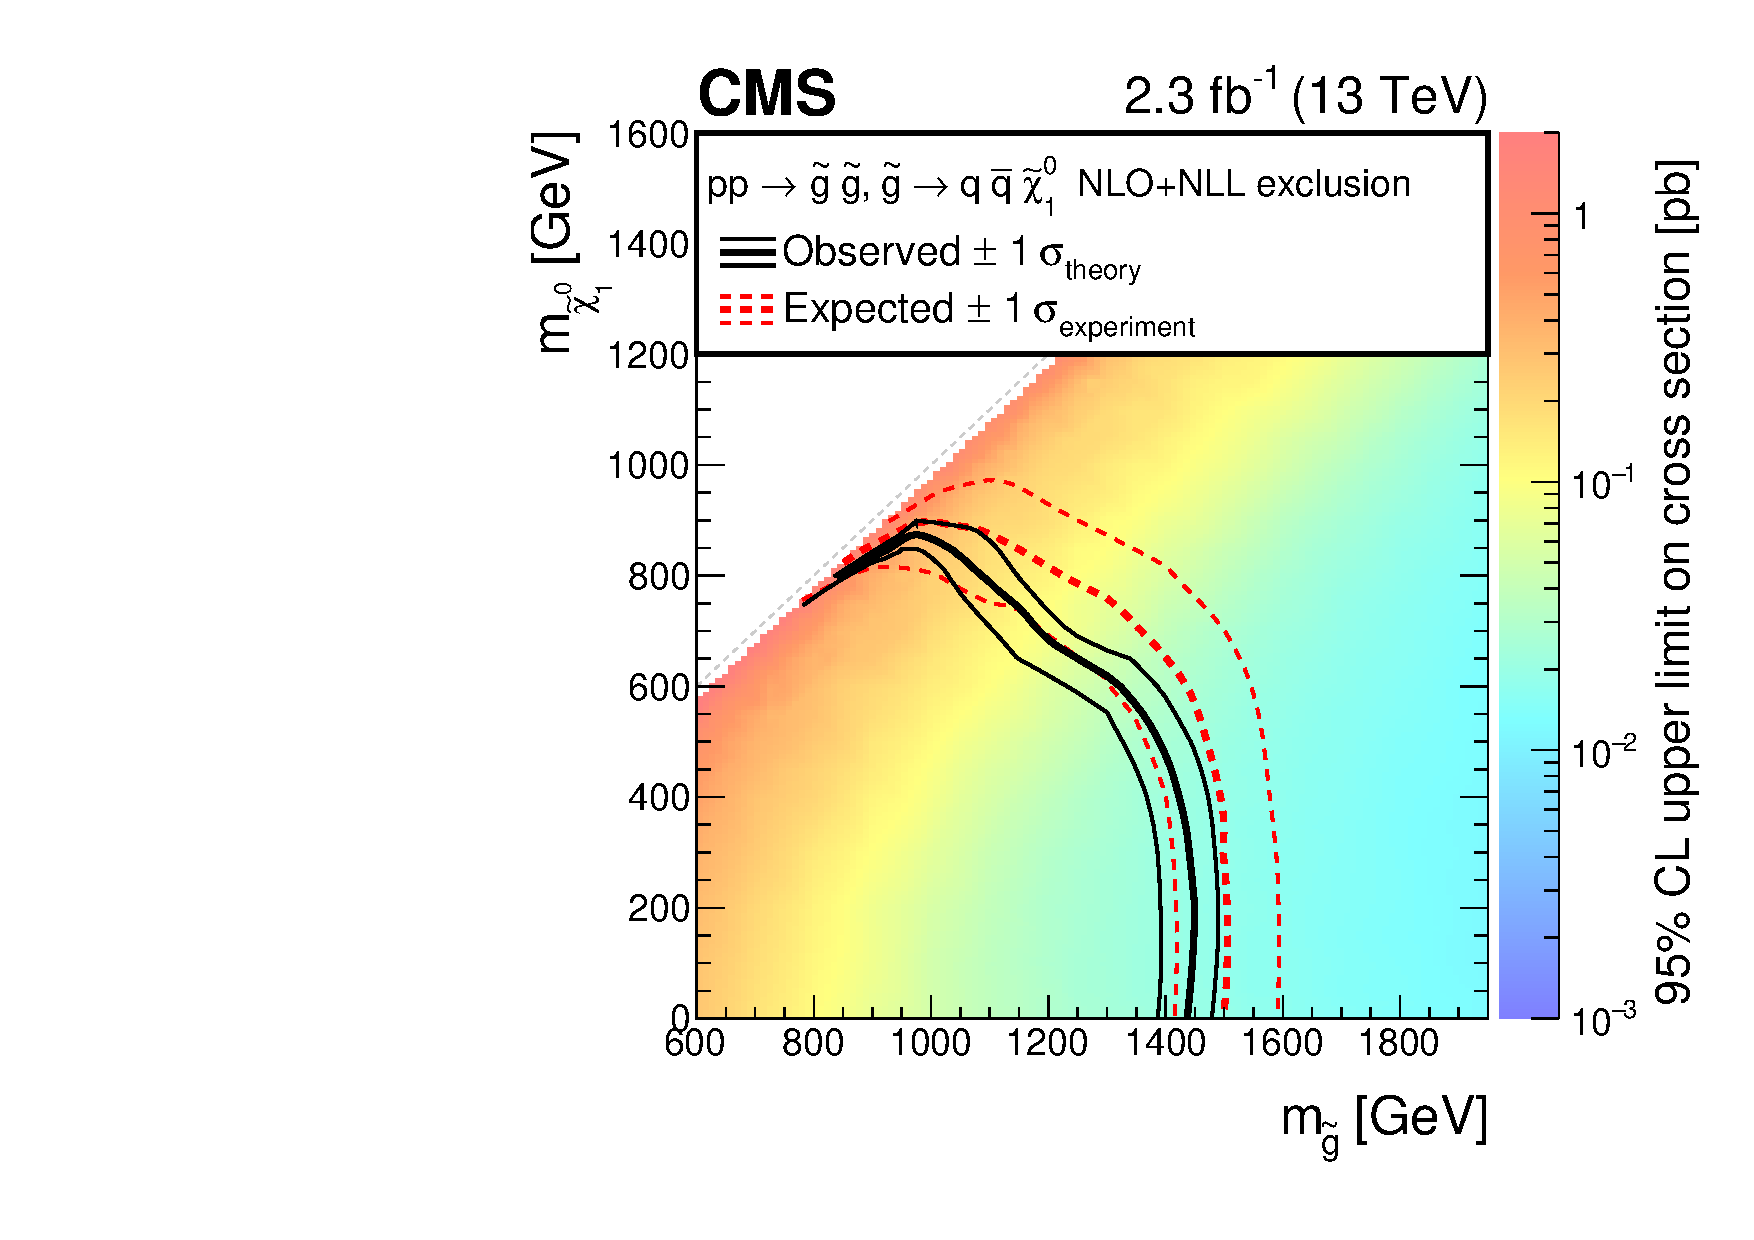
\includegraphics[width=0.48\textwidth]{figures/SusySearches/Ra2b2015/SMSqqqqXSEC.pdf}
    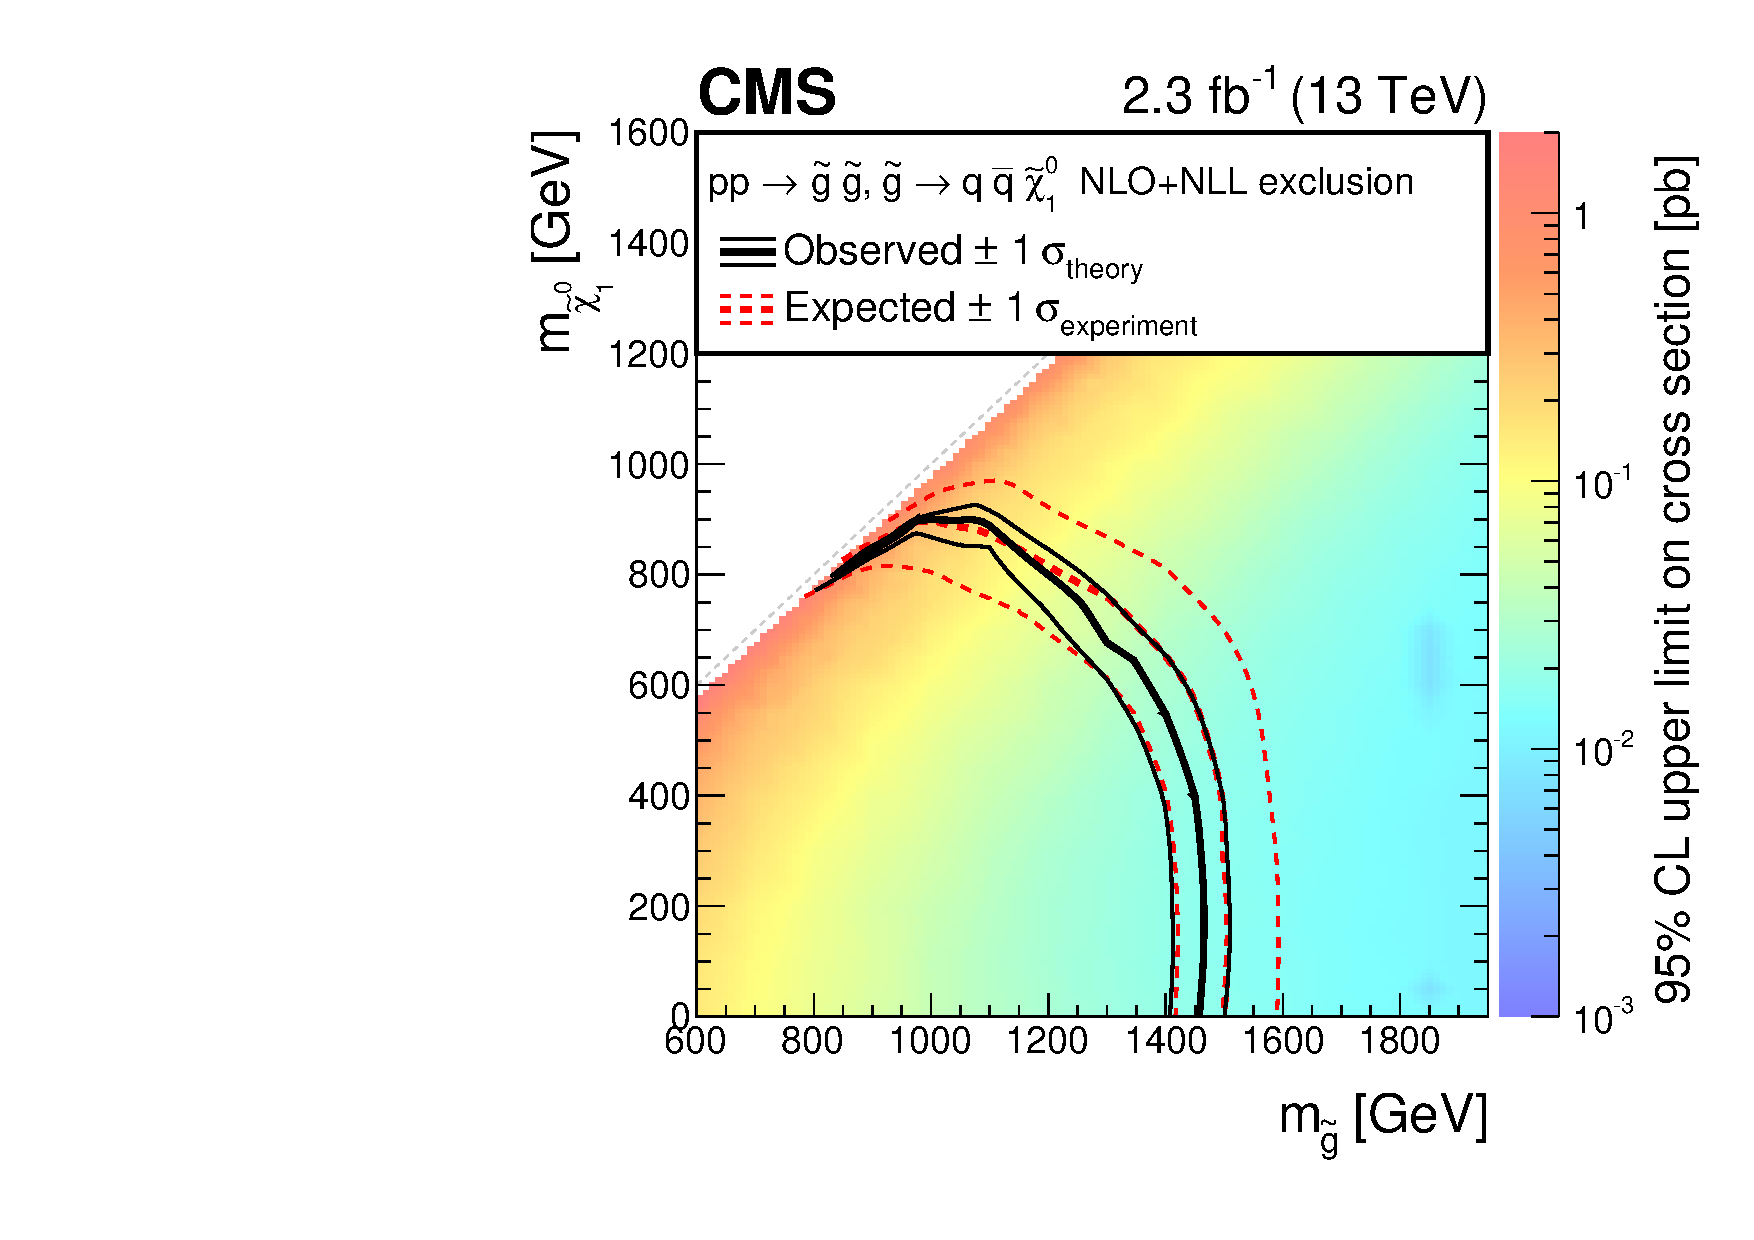
\includegraphics[width=0.48\textwidth]{figures/SusySearches/Ra2b2015/SMSqqqqXSEC_rps.pdf}
    \caption{Observed (black contour) and expected (red contour) limits on the masses of the gluino and LSP using the QCD estimate based on the inverted $\Delta\phi$ method (left) and the rebalance and smear method (right), in the context of the T1qqqq model. The dashed (grey) lines indicate the $\tilde{\chi}^{0}_{1}=m_{\tilde{\text{g}}}$ diagonal.}
    \label{fig:limitsT1qqqq}
\end{figure*}
\begin{figure*}[tb!]
\centering
    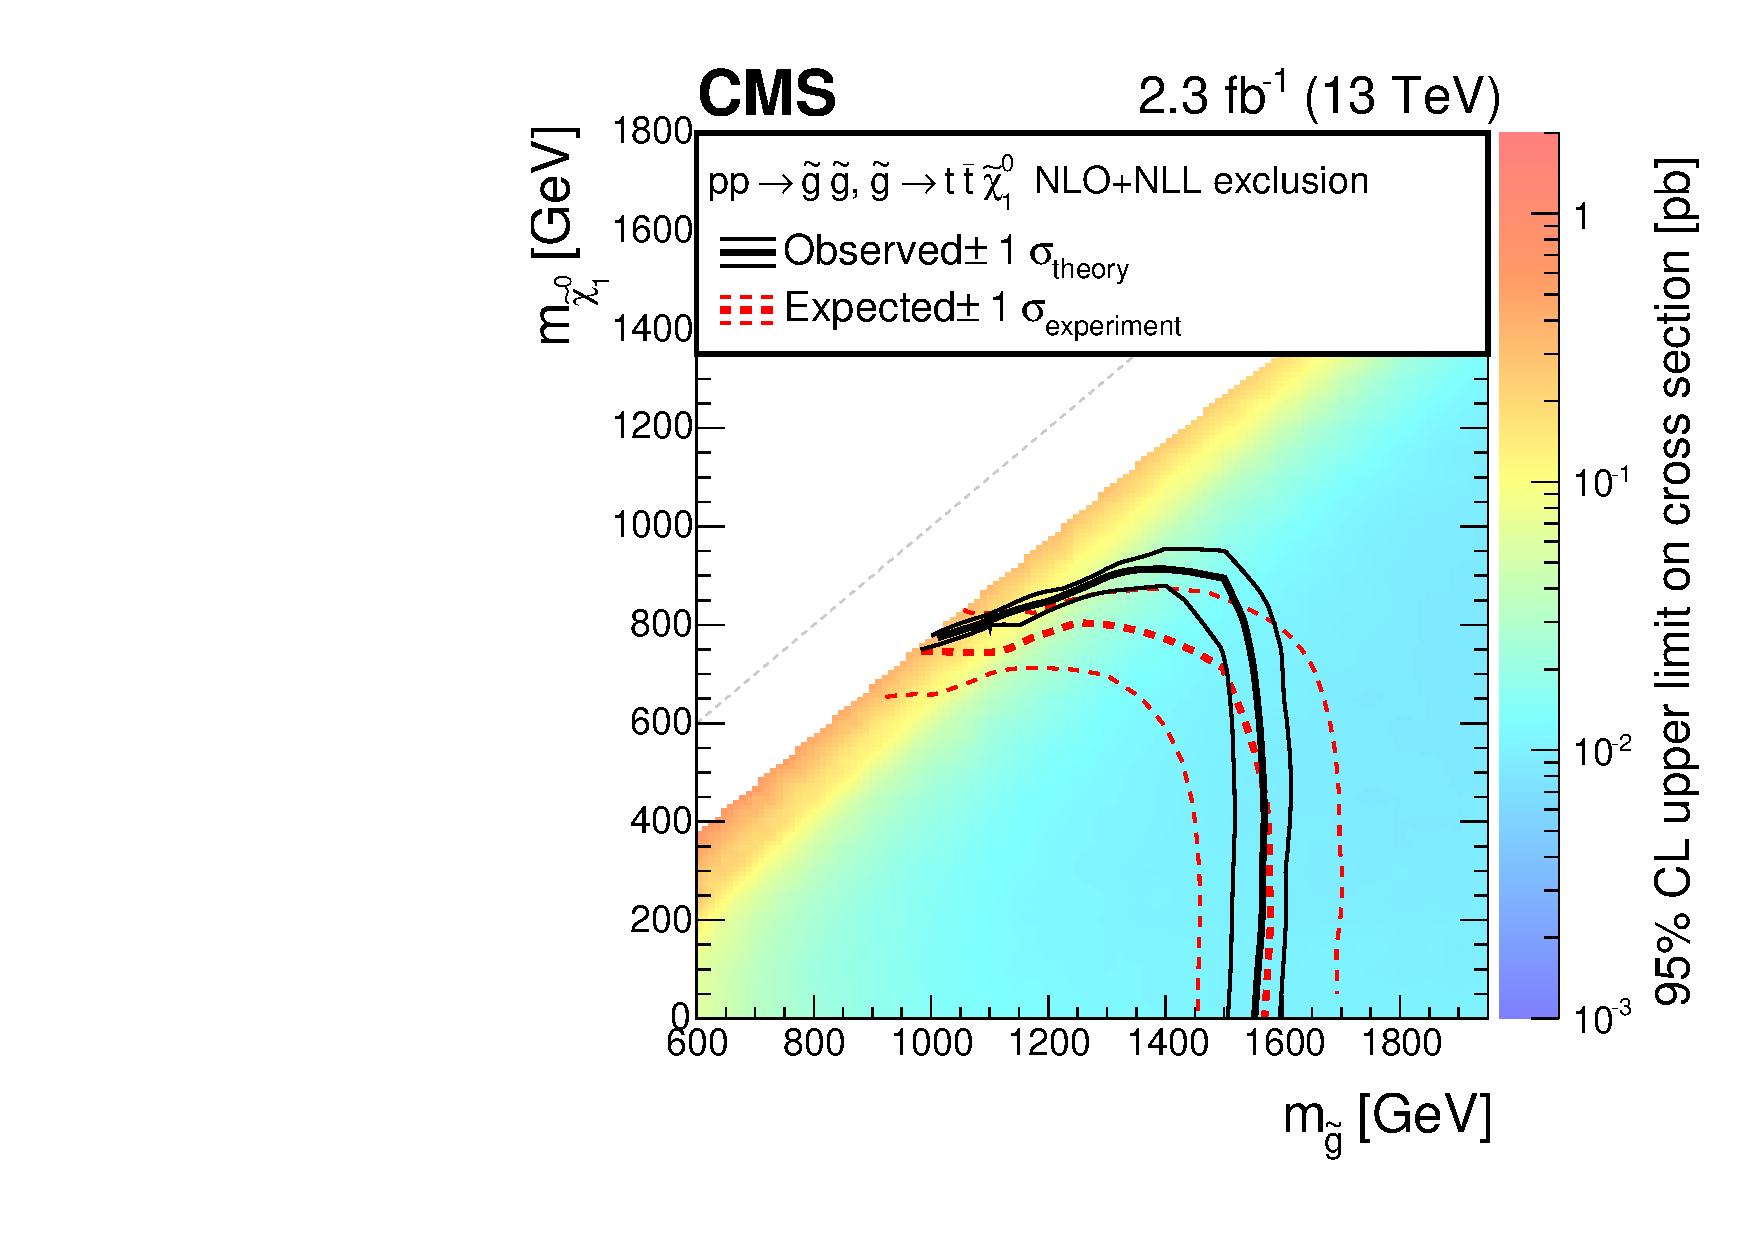
\includegraphics[width=0.48\textwidth]{figures/SusySearches/Ra2b2015/SMSttttXSEC.pdf}
    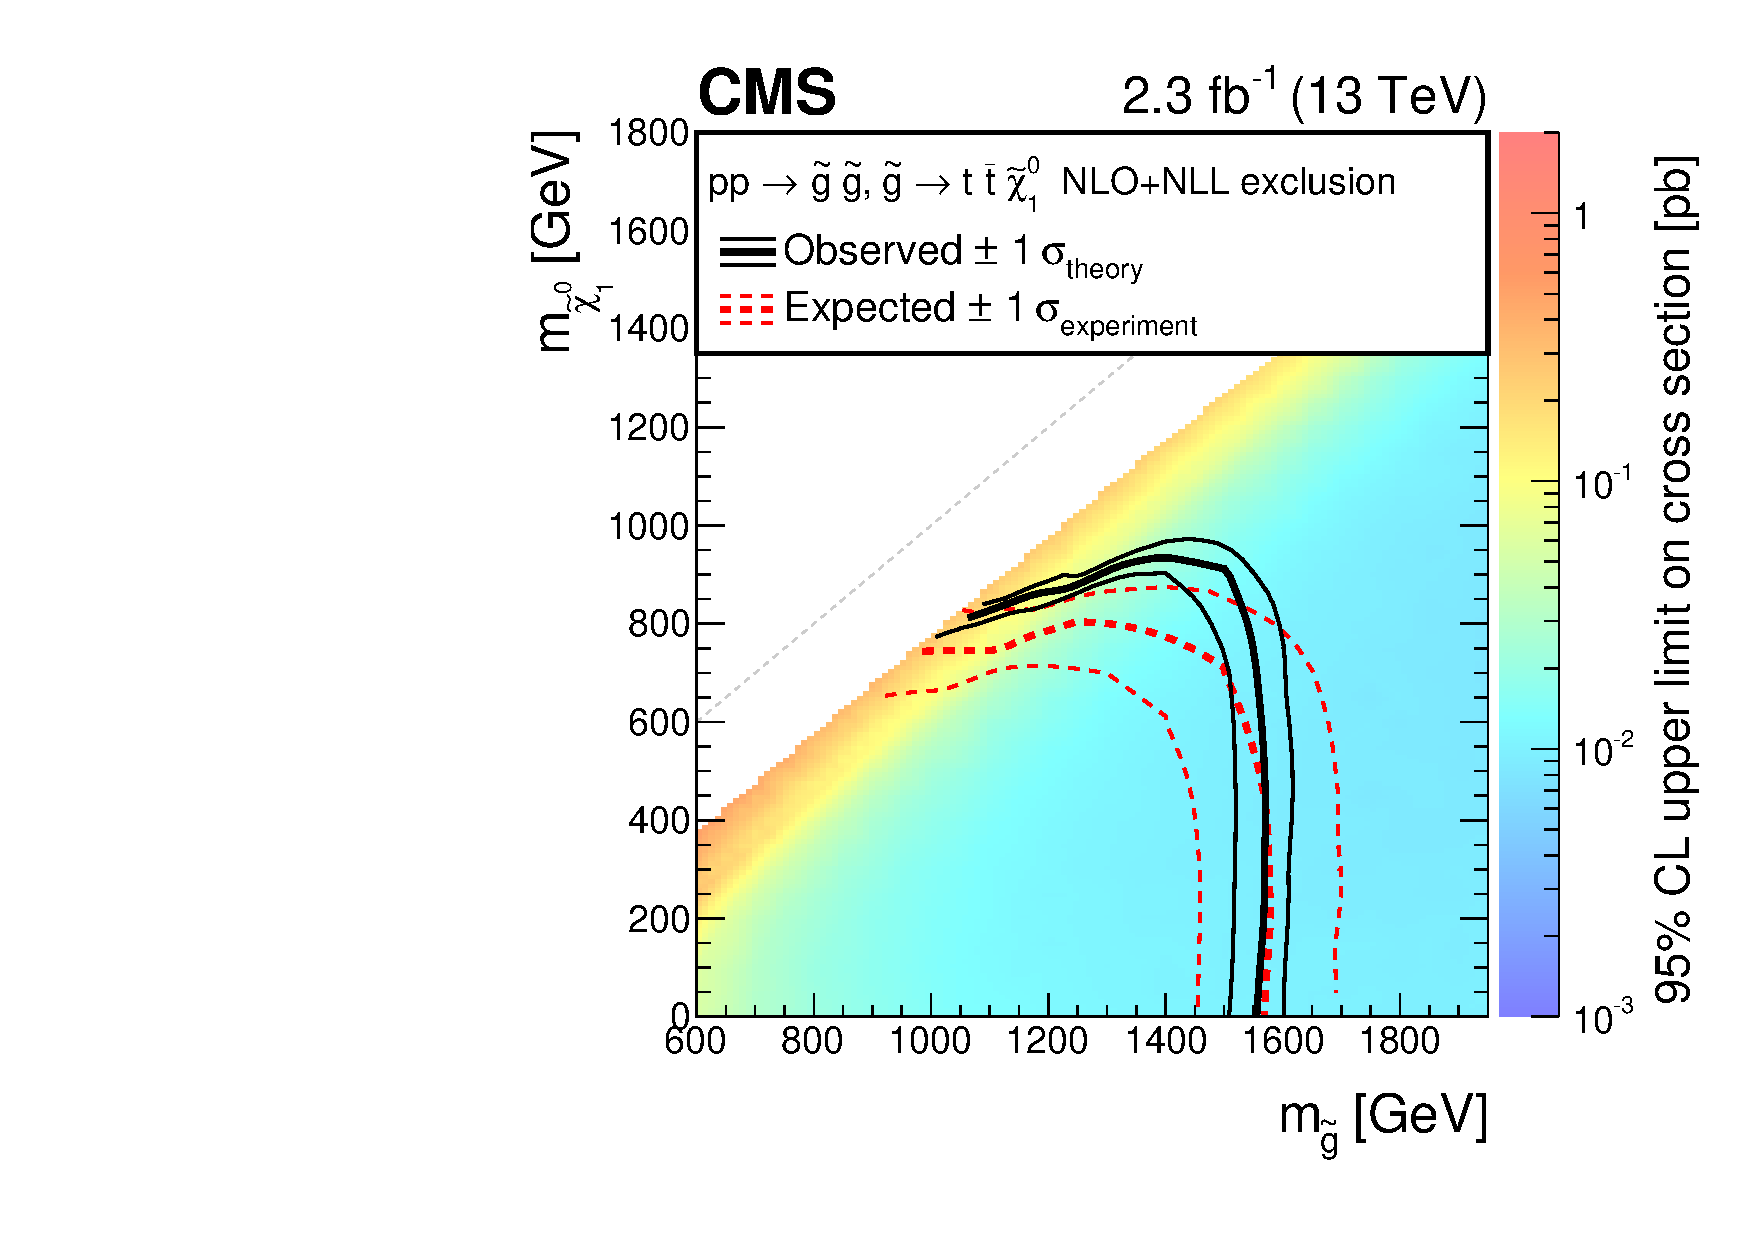
\includegraphics[width=0.48\textwidth]{figures/SusySearches/Ra2b2015/SMSttttXSEC_rps.pdf} \\
    \caption{Observed (black contour) and expected (red contour) limits on the masses of the gluino and LSP using the QCD estimate based on the inverted $\Delta\phi$ method (left) and the rebalance and smear method (right), in the context of the T1tttt model.}
    \label{fig:limitsT1tttt}
\end{figure*}
\begin{figure*}[tb!]
\centering
    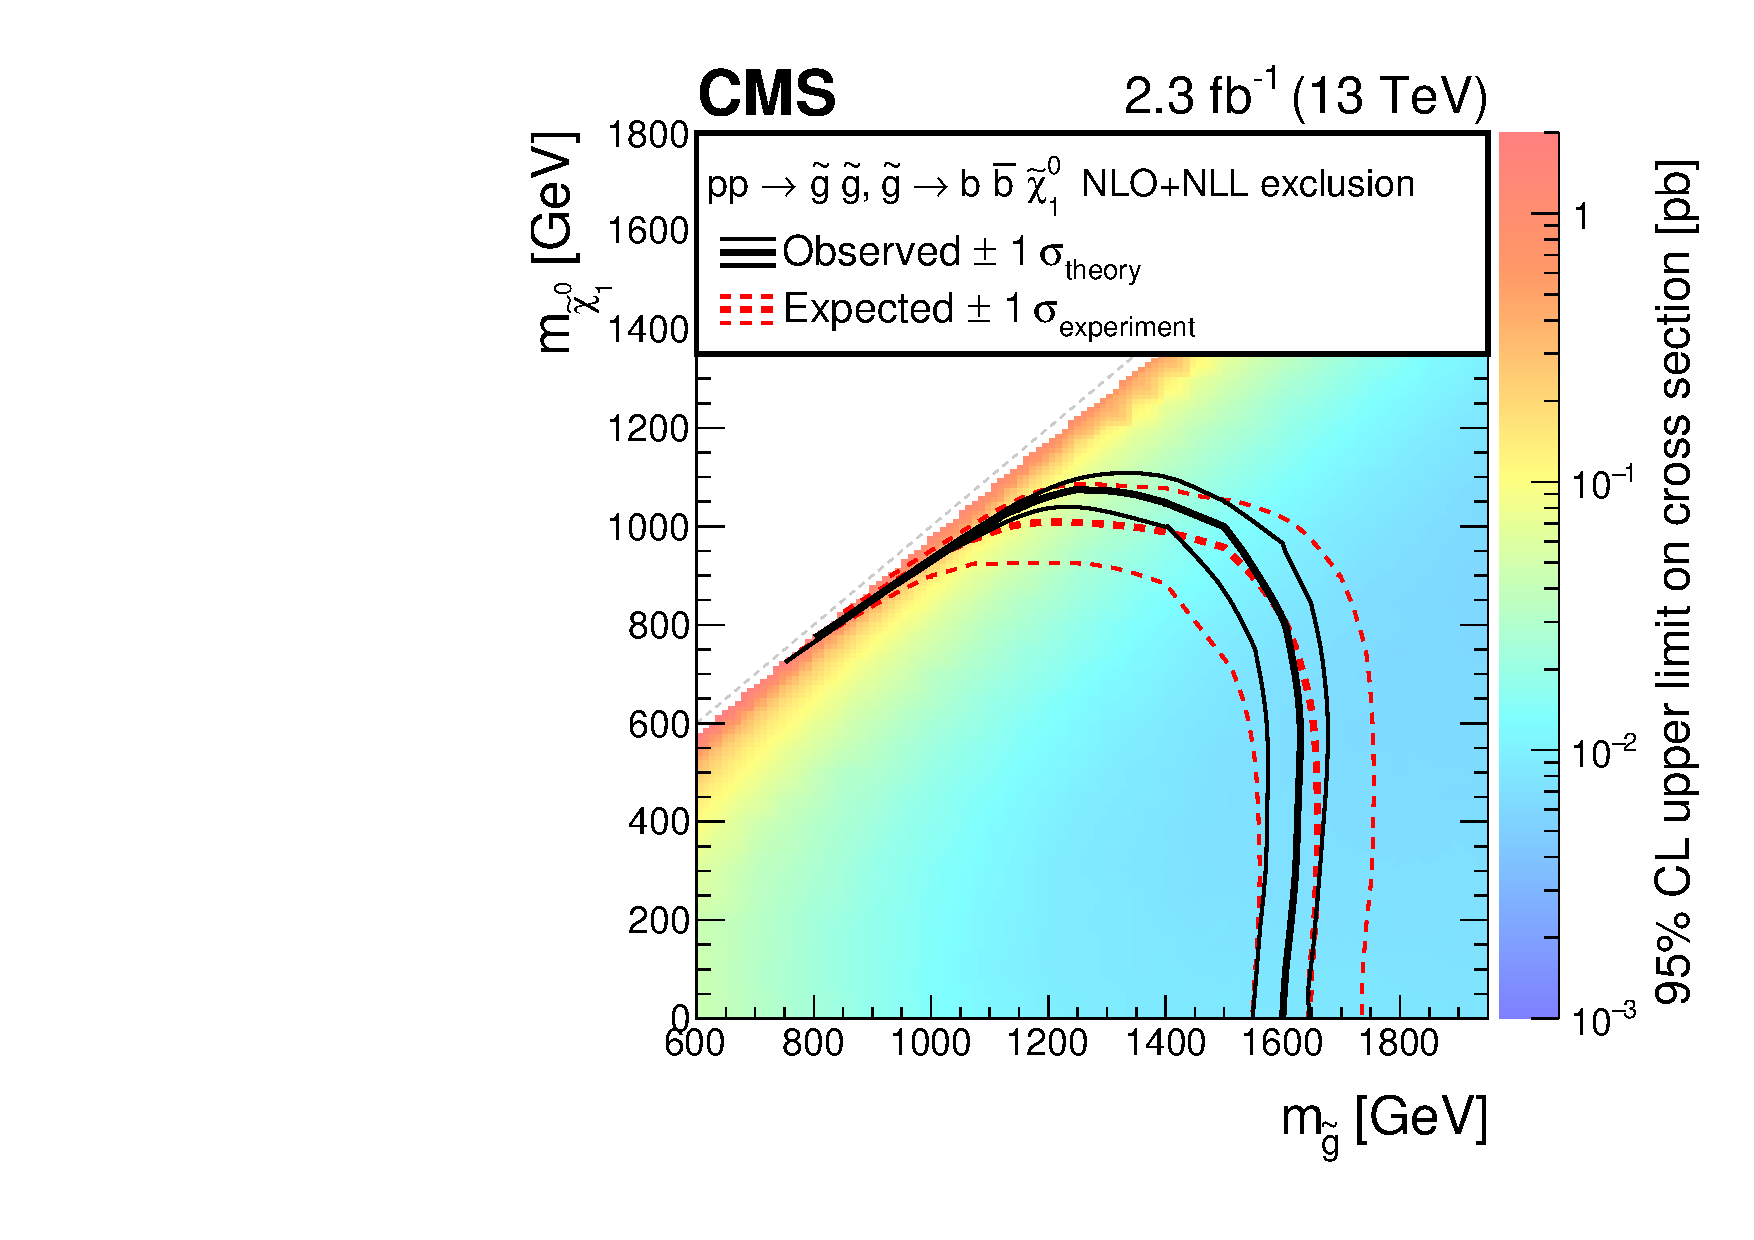
\includegraphics[width=0.48\textwidth]{figures/SusySearches/Ra2b2015/SMSbbbbXSEC.pdf}
    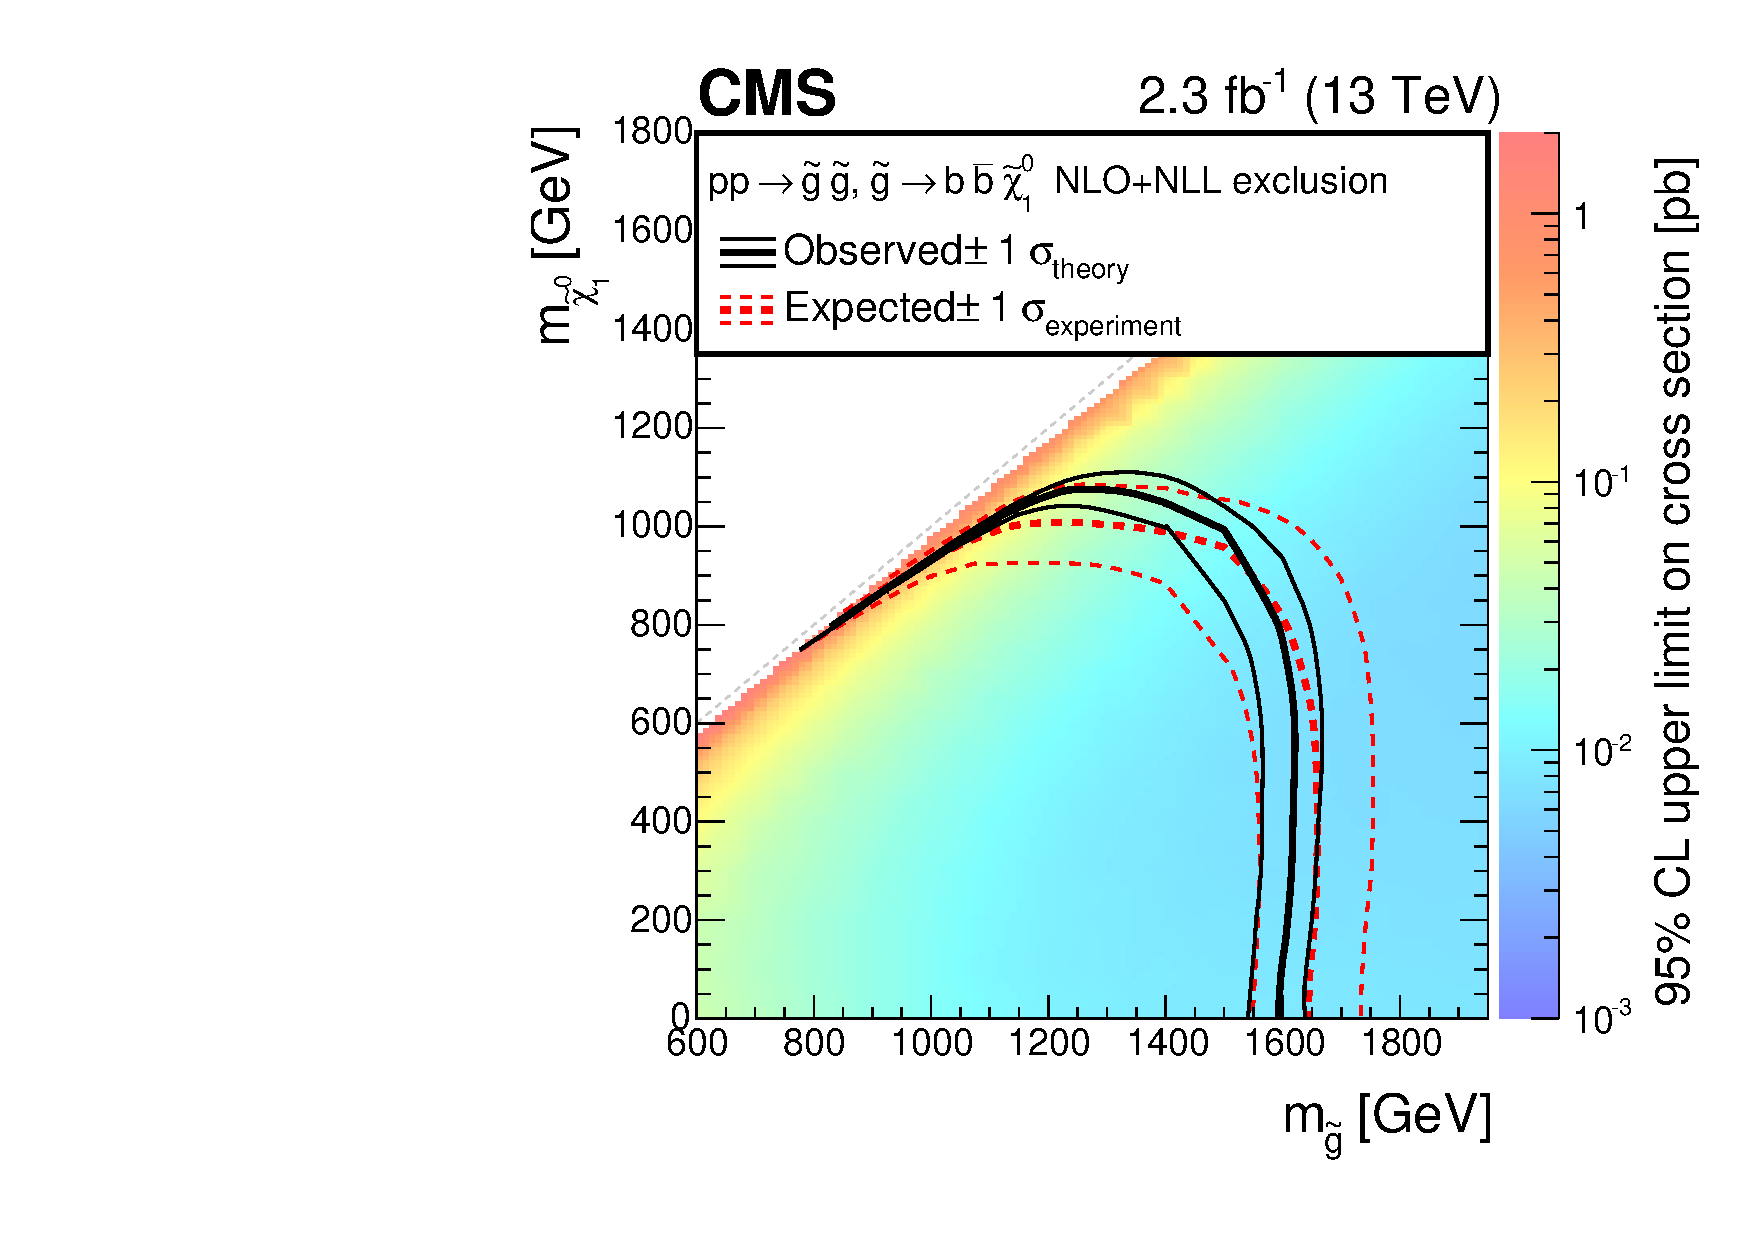
\includegraphics[width=0.48\textwidth]{figures/SusySearches/Ra2b2015/SMSbbbbXSEC_rps.pdf} \\
    \caption{Observed (black contour) and expected (red contour) limits on the masses of the gluino and LSP using the QCD estimate based on the inverted $\Delta\phi$ method (left) and the rebalance and smear method (right), in the context of the T1bbbb model.}
    \label{fig:limitsT1bbbb}
\end{figure*}
\begin{figure*}[tb!]
\centering
    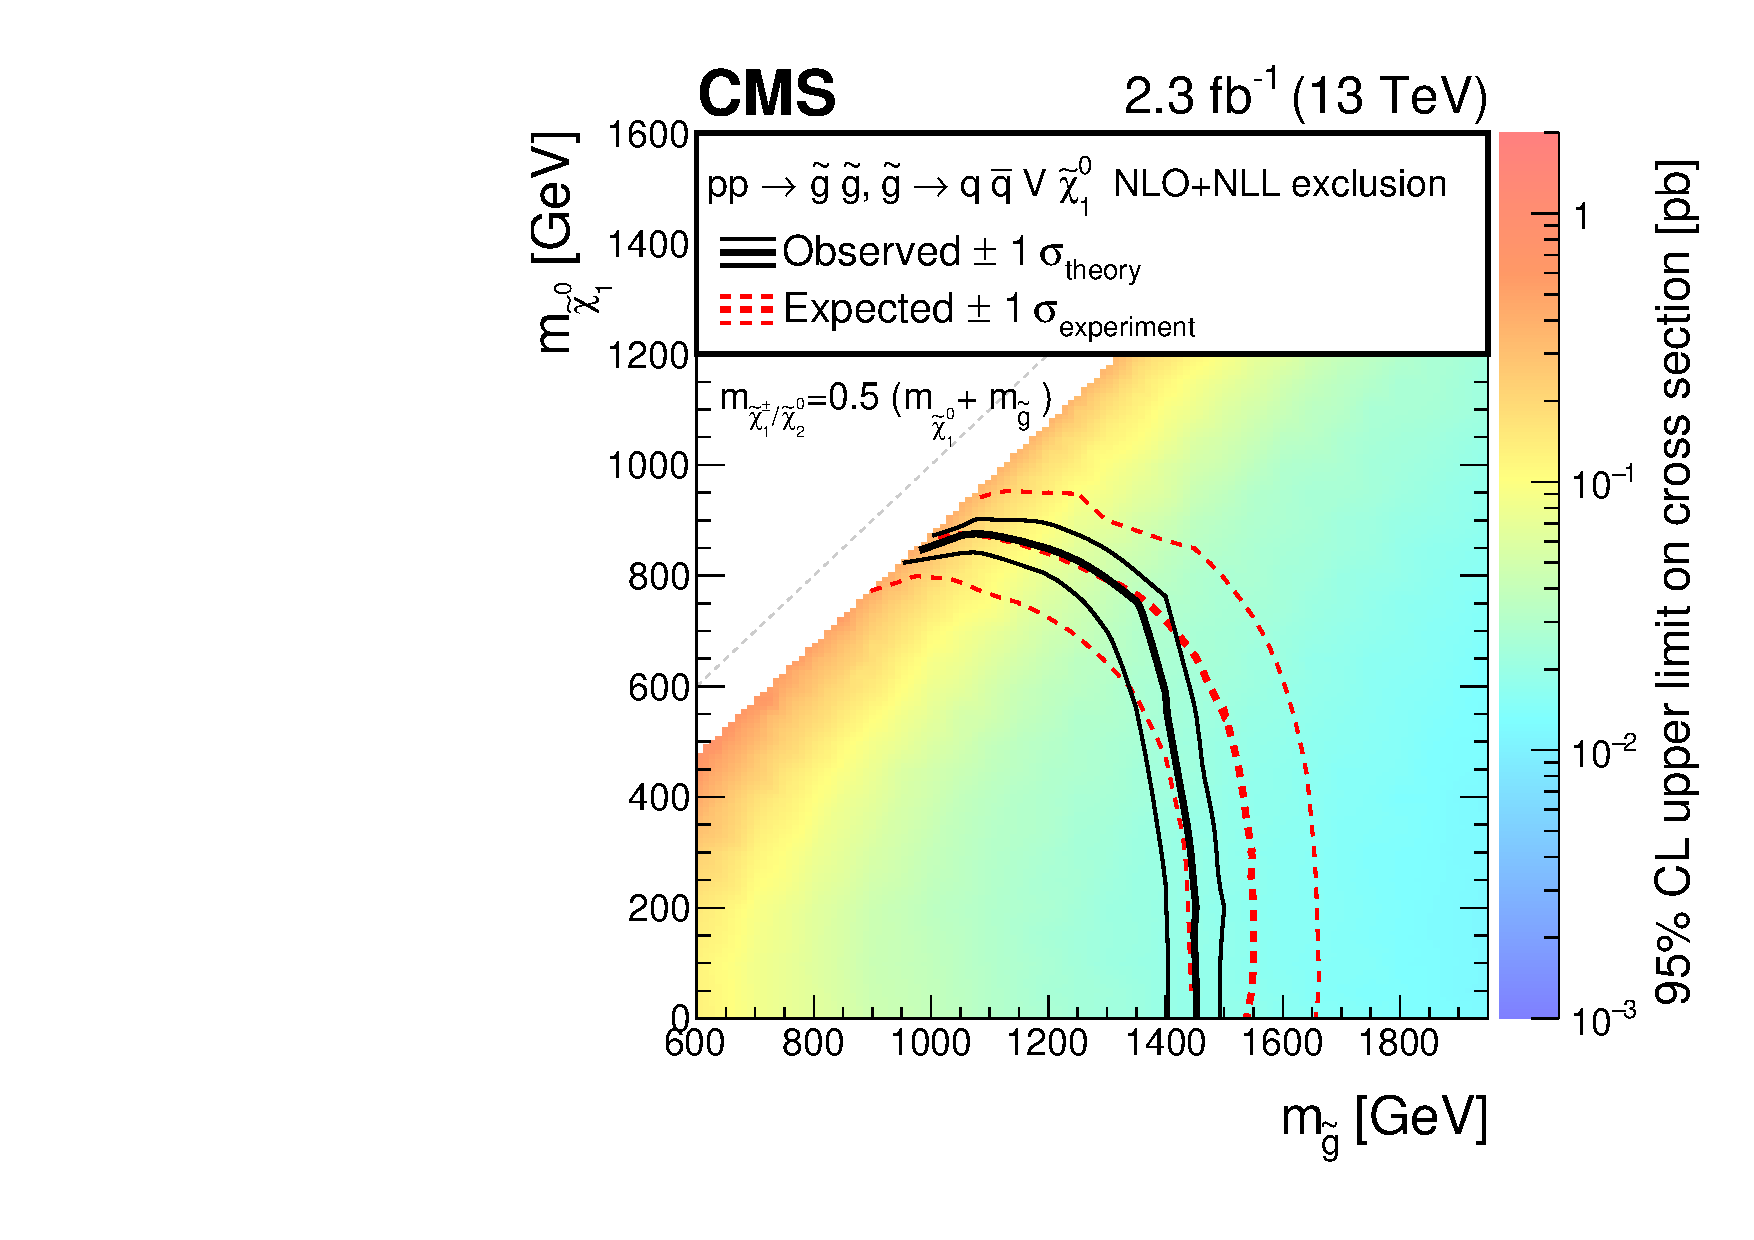
\includegraphics[width=0.48\textwidth]{figures/SusySearches/Ra2b2015/SMSqqqqVVXSEC.pdf}
    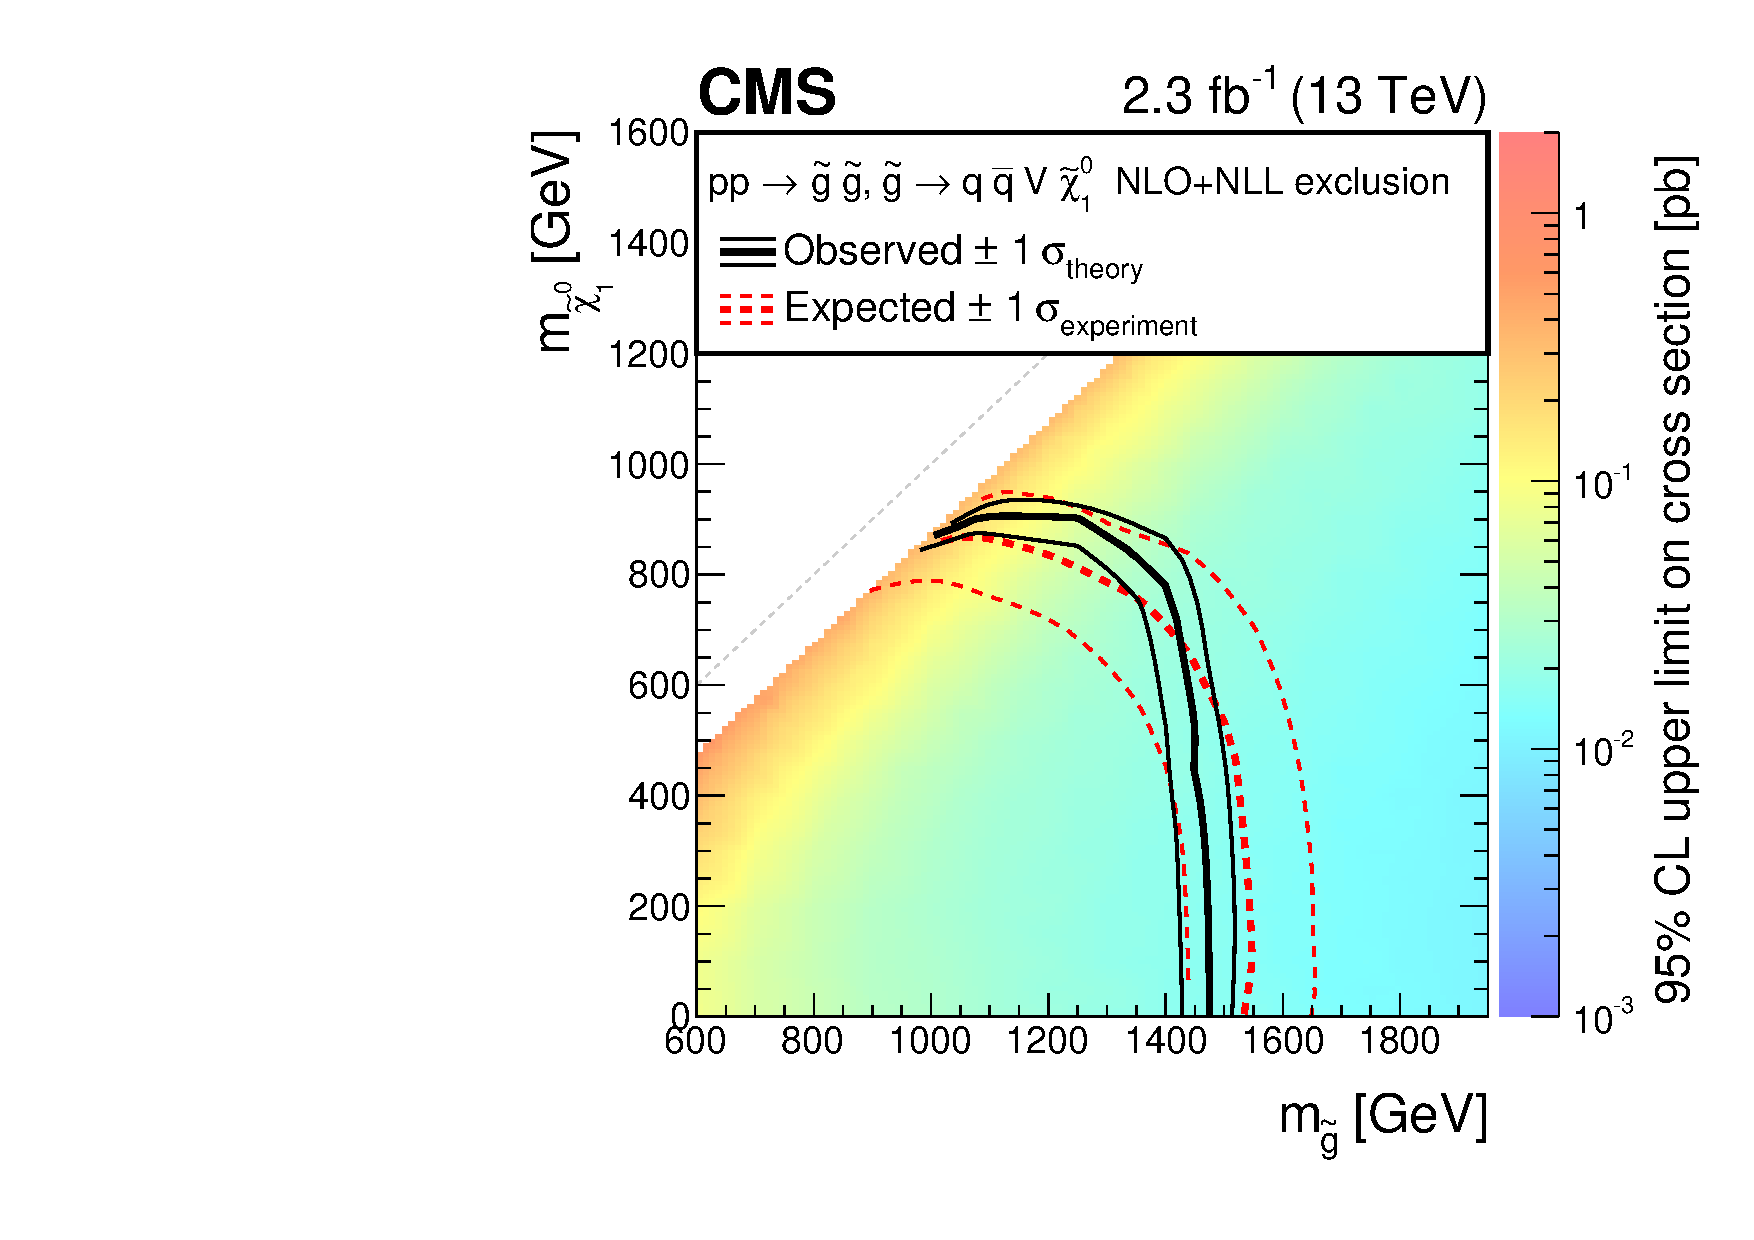
\includegraphics[width=0.48\textwidth]{figures/SusySearches/Ra2b2015/SMSqqqqVVXSEC_rps.pdf}
    \caption{The observed (black contour) and expected (red contour) limits on the masses of the gluino and LSP using the QCD estimate based on the inverted $\Delta\phi$ method (left) and the rebalance and smear method (right), in the context of the T5VV model. }
    \label{fig:limitsT5vv}
\end{figure*}

